%---------------------------------------------------------------------------%
%-                                                                         -%
%-                           LaTeX Template                                -%
%-                                                                         -%
%---------------------------------------------------------------------------%
%- Copyright (C) Huangrui Mo <huangrui.mo@gmail.com>
%- This is free software: you can redistribute it and/or modify it
%- under the terms of the GNU General Public License as published by
%- the Free Software Foundation, either version 3 of the License, or
%- (at your option) any later version.
%---------------------------------------------------------------------------%
%->> Document class declaration
%---------------------------------------------------------------------------%
\documentclass[doublesided]{Style/ucasthesis}%
%- Multiple optional arguments:
%- [<singlesided|doublesided|printcopy>]% set one or two sided eprint or print
%- [draftversion]% show draft version information
%- [fontset=<fandol|...>]% specify font set to replace automatic detection
%- [scheme=plain]% thesis writing of international students
%- [standard options for ctex book class: draft|paper size|font size|...]%
%---------------------------------------------------------------------------%
%->> Document settings
%---------------------------------------------------------------------------%
\usepackage[authoryear,myhdr,list]{Style/artratex}% document settings
%- usage: \usepackage[option1,option2,...,optionN]{artratex}
%- Multiple optional arguments:
%- [bibtex|biber]% set bibliography processor and package
%- [<numbers|super|authoryear|alpha>]% set citation and reference style
%- <numbers>: textual: Jones [1]; parenthetical: [1]
%- <super>: textual: Jones superscript [1]; parenthetical: superscript [1]
%- <authoryear>: textual: Jones (1995); parenthetical: (Jones, 1995)
%- <alpha>: textual: not available; parenthetical: [Jon95]
%- [geometry]% reconfigure page layout via geometry package
%- [lscape]% provide landscape layout environment
%- [myhdr]% enable header and footer via fancyhdr package
%- [color]% provide color support via xcolor package
%- [background]% enable page background
%- [tikz]% provide complex diagrams via tikz package
%- [table]% provide complex tables via ctable package
%- [list]% provide enhanced list environments for algorithm and coding
%- [math]% enable some extra math packages
\usepackage{Style/artracom}% user defined commands
\usepackage{url}
\usepackage{bbm}
\usepackage{mathrsfs}
\usepackage{float}
\usepackage{hyperref}
\usepackage{multirow}
\usepackage{algorithm}
%\usepackage{algorithmic}
%---------------------------------------------------------------------------%
%->> Document inclusion
%---------------------------------------------------------------------------%
%\includeonly{Tex/Chap_1,...,Tex/Chap_N}% selected files compilation
%---------------------------------------------------------------------------%
%->> Document content
%---------------------------------------------------------------------------%
\begin{document}
%-
%-> Frontmatter: title page, abstract, content list, symbol list, preface
%-
\frontmatter% initialize the environment
%---------------------------------------------------------------------------%
%->> Titlepage information
%---------------------------------------------------------------------------%
%-
%-> Chinese titlepage
%-
\confidential{}% confidential level
\schoollogo{scale=0.095}{ucas_logo}% university logo
\title{基于强化学习的文本语义匹配}% \title[short title for headers]{Long title of thesis}
\author{何逸轩}% name of author
\advisor{徐君\hspace{1em}研究员}% supervisor
\advisorsec{}% co-supervisor
\degree{硕士}% degree
\degreetype{工学}% degree type
\major{计算机软件与理论}% major
\institute{中国科学院计算技术研究所}% institute of author
\chinesedate{二〇一八年五月}% customized date, 6 for summer and 12 for winter graduation
%-
%-> English titlepage
%-
\englishtitle{The Text Semantic Matching based on\\ Reinforcement Learning}
\englishauthor{He Yixuan}
\englishadvisor{Xu Jun}
\englishdegree{Master}% degree type <Doctor|Master> of <Philosophy|Natural Science|Engineering>
\englishdegreetype{Science}
\englishthesistype{thesis}% thesis type <thesis|dissertation>
\englishmajor{Computer Software and Theory}% major
\englishinstitute{Institute of Computing Technology\\Chinese Academy of Sciences}
\englishdate{May, 2018}% customized date
%-
%-> Create titlepages
%-
\maketitle
\makeenglishtitle
%-
%-> Author's declaration
%-
\makedeclaration
%-
%-> Chinese abstract
%-
\chapter*{摘\quad 要}
\chaptermark{摘\quad 要}
\setcounter{page}{1}% set page number
\pagenumbering{Roman}% set large roman

文本匹配是自然语言处理重要的基础问题之一,许多自然语言处理中的任务例如信息获取,问答系统,机器翻译,对话系统等等,都可以被视为文本匹配问题。
在工业界,网页搜索,新闻推荐等等领域都需要文本匹配算法。

传统的文本匹配算法往往基于人工抽取的规则进行模式匹配,这导致规则复杂而且难以管理;因此目前对文本匹配的研究大都试图通过深度神经网络理解文本语义进行语义匹配。
但是目前计算机仍然难以理解人类的语义,这种基于语义的匹配具有天然的劣势。

强化学习的出现给基于模式的文本匹配带来了新的可能性。通过强化学习建模人工抽取的规则,可以解决传统的文本匹配算法的问题。

通过调研,本文发现利用强化学习进行文本匹配的主要难题在于:

(1) 如何设计文本匹配的策略和奖励机制

(2) 如何解决传统模式匹配的固有难点、

(3) 如何提升算法的训练和推导速度

本文的主要工作是利用强化学习建模文本匹配并解决上面的挑战。
首先,本文针对于文本匹配的场景设计了高效的策略和奖励机制,使得强化学习可以有效的解决文本匹配的问题;
然后,本文对于传统的模式匹配难以解决的问题如词语顺序,对强化学习算法进行调整,使其可以有效解决这些问题;
最后,针对强化学习运行速度慢、难以加速等问题,本文针对匹配场景进行了算法优化,大大提升了算法的运行速度。
本文提出的模式文本匹配模型是一种高效的文本匹配算法。

\keywords{文本匹配, 强化学习, AlphaGo Zero}
%-
%-> English abstract
%-
\chapter*{Abstract}
\chaptermark{Abstract}

Text matching is one of the most important problems in nature language processing, many tasks like information retrive, question answer, machine translation and dialogue can be formalized as text matching.
Text matching plays a key role in web searching and news recommadation.
Traditional text matching research is often based on manually extracted rules for pattern matching, which leads to complex rules and difficult management. So currently almost all search concentrates on semantic match based on deep learning. But it is still very hard to make machine understand semantics, so this kind of methods have intrinsic weakness.

In this paper, we found the main troubles in the pattern text matching based on reinforcement learning are:

(1) how to design reward and policy function for text matching

(2) how to solve intrinsic problems in traditional text matching

(3) how to speed up model training and inference

In order to solve the problems addressed above, we introduced how to improve text matching performance by reinforcement learning:
First, we introduced a effective policy and value function which make reinforcement learning can solve text matching problems efficiently
Second, in order to be solving some problems in traditional pattern matching such as word order more effectively, we adjusted the reinforcement learning algorithm.
Last, we optimized our model to decrease running time in the matching situation.

Our model is high-performance, real-time and has the ability to evolve.

\englishkeywords{Text Matching, Reinforcement Learning, AlphaGo Zero}
%---------------------------------------------------------------------------%
% title page, abstract, dedication
{% content list region
\linespread{1.2}% local line space
%\intotoc{\contentsname}% add link to contents table and bookmark
\tableofcontents% contents catalog
%\intotoc{\listfigurename}% add link to contents table and bookmark
\listoffigures% figures catalog
%\intotoc{\listtablename}% add link to contents table and bookmark
\listoftables% tables catalog
}
\input{Tex/Prematter}% list of symbols, preface content
%-
%-> Mainmatter
%-
\mainmatter% initialize the environment
%---------------------------------------------------------------------------%
%->> Main content
%---------------------------------------------------------------------------%

\chapter{引言}
\label{chap:introduction}

\section{研究背景}
近二十年来,计算机以及智能终端的计算和存储能力都得到了巨大的飞跃,互联网的信息量也呈现出爆炸式的增长。互联网的发展不仅为计算机技术带来许多新的问题和场景,同样给活在信息时代的人们提出了巨大的挑战。在每天生成的大量数据面前,如何高效的筛选出自己需要的信息成了大多人都需要面对的问题。据统计\citep{website:WWW},目前最主要的搜索引擎google每天新增的网页量高达40亿。

\begin{figure}[!htbp]
    \centering
    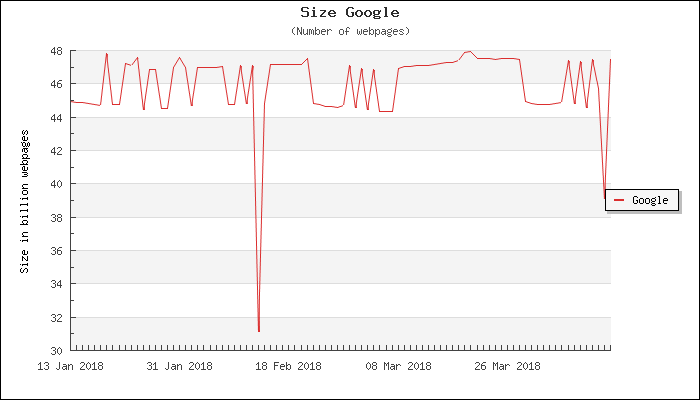
\includegraphics[width=0.80\textwidth]{google}
    \bicaption{google 2018年1-3月网页增长量}{The increment of web page indexed by google between 2018.1 to 2018.3}
    \label{fig:user-ad-match}
\end{figure}

数据量的增长不仅意味着高效的信息获取变得困难,同样意味着会有大量重复冗余的信息生成。如何去除冗余的信息,同样是一个巨大的问题。

文本长期以来一直都是人类信息传播的主要载体。人类大部分的知识都是以文本的形式进行记录和传播的,而人类自幼就开始学习如何从文本中获取信息,虽然互联网的发展大大促进了视频和语音的传递,但是文本仍然是大多数人获取信息的高效和主要手段。而文本匹配作为信息检索和冗余文本消除的基础,在各大互联网公司得到了广泛的使用。

\begin{figure}[!htbp]
    \centering
    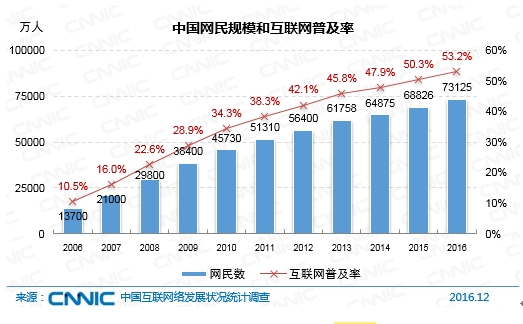
\includegraphics[width=0.80\textwidth]{CNNIC}
    \bicaption{中国网民和互联网普及率}{Chinese internet users and internet penetration rate}
    \label{fig:CNNIC}
\end{figure}

不仅如此,在自然语言处理中,需要任务如信息获取,问答系统,机器翻译,对话系统等等,都不同程度的需要用到文本匹配技术。根据使用场景的不同,文本匹配可以被分为三类:短文本-短文本匹配,短文本-长文本匹配以及长文本-长文本语义匹配。

1. 短文本-短文本匹配

短文本-短文本的匹配被广泛使用在工业界。如网页搜索中,搜索引擎必须计算用户的查询(query) 和网页标题(web page title)的语义相关性,并在此基础上结合用户画像进行排序返回给用户;在知乎,Quora等问答网站上需要进行相似问题的合并,这时我们需要度量一个问题和其他问题之间的相似度。这些场景都需要短文本-短文本的匹配作为基础。

\begin{figure}[!htbp]
    \centering
    
\includegraphics[width=1.0\textwidth]{ques_red}
    \bicaption{知乎问题重定向}{Question redirection in zhihu}
    \label{fig:ques_red}
\end{figure}

以相似问题的检测为例,对于两个给定的问题,我们用一个函数映射 $f:x\to \mathbb{R}^k$ 将句子中的每个词映射到一个高维的向量空间,得到句子的矩阵映射。在句子矩阵映射的基础上,我们可以选择利用深层网络建模单个句子的语义信息,或者直接利用深层网络建模句子之间的交互信息,最后将两个句子的语义信息或者句子的交互信息映射成一个一维的概率表达。

2. 短文本-长文本匹配

短文本-长文本语义匹配同样在在工业界被广泛运用,信息检索就是典型的短文本-长文本的匹配场景。这种场景中我们需要首先利用倒排索引等手段对网页正文建立索引,根据用户的输入利用事先建立的索引初步召回候选文档;然后利用文本匹配算法计算用户输入的查询和候选文档的相似度。在计算用户查询和网页正文的语义相关度时,由于用户查询通常较短,而网页正文较长,因此查询与正文的匹配与上文提到的短文本-短文本不同,通常需要使用短文本-长文本语义匹配,以得到更好的匹配效果。在计算相似度的时候,我们规避对短文本直接进行主题映射,而是根据长文本的主题分布,计算该分布生成短文本的概率,作为它们之间的相似度。
利用匹配算法计算出的相似度结合用户画像等排序得到最后的结果呈现给用户。

用于长文本相比于短文本的语义更加丰富,段落之间层次化的组织结构以及上下之间的语义关系使得短文本-长文本的匹配问题更加复杂。

3. 长文本-长文本匹配
由于长文本的语义丰富,上下文之间语义关系负责,因此长文本-长文本的匹配往往基于自动摘要或者主题模型等等方式,将长文本压缩到相同的高维空间,通过高维空间的距离衡量2个文本的相似度。高维空间的距离可以利用Hellinger Distance\citep{website:Hellinger}和Jensen-Shannon Divergence(JSD)\citep{website:Shannondivergence}。长文本-长文本的匹配往往用于新闻推荐等领域。

\begin{figure}[!htbp]
  \centering
  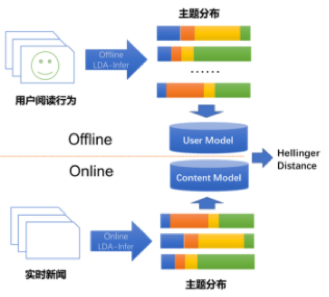
\includegraphics[width=0.6\linewidth]{news_com}
  \caption{新闻个性化推荐}{news recommendation}
  \label{fig:news_recom}
\end{figure}

\section{研究意义}
文本匹配是自然语言处理的重要问题,在信息检索、广告计算等领域有着广泛的应用,网页搜索,相似问题合并等等都需要文本匹配作为基础。早期的文本匹配算法往往是对词向量空间如VSM,BM25等的匹配,主要解决基于词汇层面的匹配问题。但是基于词汇层面的匹配只能解决词汇的相似,很难处理语义匹配;同时算法的泛化能力不足,在面对新任务时,必须重新设计特征和算法。

一个优秀的文本匹配算法必须要解决以下三个问题:

1. 语言多义性。相同的词语在不同语境下可能拥有不同的含义,如 “苹果” 既可以表示水果,也可以表示科技公司;而不同的词语也可以表达相同的语义,如 “出租车”,“的士”。

2. 语言的组合结构。由相同词语组成的句子由于语序的不同,也可能产生不同的语义。例如 “机器学习” 和 “学习机器”。

3. 匹配的非对称性问题。文本匹配任务并不一定要求语言相似,例如网页搜索中的查询和网页;也不一定要求语义上的相似,例如问答系统。

基于词汇的匹配模型显然无法解决这种问题。因此从上世纪 90 年代开始,有人开始尝试将主题模型应用于文本匹配,主题模型可以较好地表示文本的语义信息,从而弥补传统文本匹配算法的不足。但是从效果上看,他们都无法替代基于词汇的匹配方法,只能作为补充。
在世纪初,计算机的计算力和存储量开始爆炸式增长,因此开始有人尝试将深度学习应用于文本匹配算法上并且取得了较好的效果,
目前大部分的深度学习算法都试图利用神经网络理解语义信息,但是现阶段计算机仍然难以理解语义信息,因此基于语义信息的文本匹配算法目前具有天然劣势。

\begin{figure}[!htbp]
    \centering
    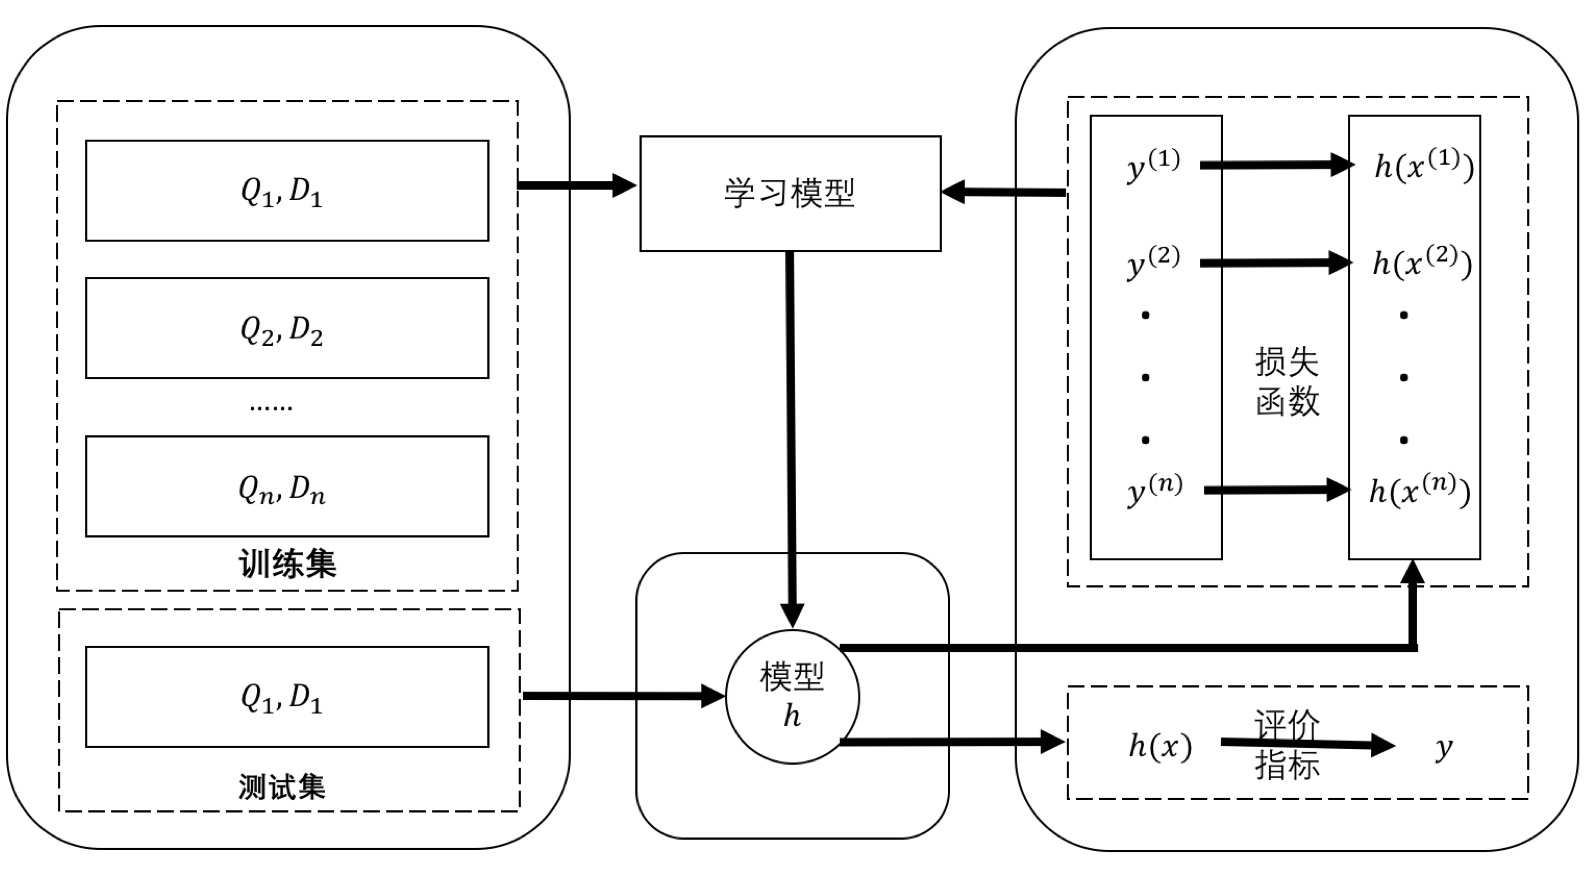
\includegraphics[width=1.0\textwidth]{match_learn_arch}
    \bicaption{文本匹配框架}{The architecture of text matching}
    \label{fig:match_learn_arch}
\end{figure}

文本匹配的算法框架如图 \ref{fig:match_learn_arch} 所示,概括了文本匹配算法中的三个主要部分:模型,数据集和评价指标。一般来说,文本匹配的数据集中正例样本为人工标注,负样本通过在整个句子空间中随机抽取句子对构成。

由于传统的模式匹配方案模式规则难以维护、系统复杂,因此近几年来对文本匹配的研究集中于深度学习,即利用深度网络学习到文本的语义信息进行匹配。但是计算机对语义理解的困难为语义匹配的方案引入了额外的复杂度,算法工程师必须进行巧妙的特征设计以应对不同的业务场景。

近几年来,深度网络极大的增强了强化学习表达能力,使得强化学习建模现实世界问题的能力越来越强。近年来,强化学习已经在游戏,围棋等等方面超越人类的表现。强化学习在规则学习方面表现出了强大的能力,部分场景下甚至可以在没有人类先验知识指导的情况下获得令人惊讶的学习能力。而文本匹配所存在的规则远远没有围棋等复杂,但是目前为止还没有人尝试利用强化学习进行文本匹配的研究,因此利用强化学习学习传统文本匹配中的规则拥有强大的潜力。

\section{本文贡献}
文本匹配是传统的自然语言处理问题,传统的基于模式匹配的方案往往规则复杂,系统难以维护;现在基于深度学习的语义匹配拥有天生的缺陷。而深度强化学习由于其强大的建模能力开始在各个场合发挥越来越重要的作用,因此利用强化学习建模模式匹配,基于大量匹配数据学习匹配规则成为一种可能。本文分析了文本匹配场景下的文本数据特点以及传统文本匹配规则的基础上,提出了基于强化学习的文本匹配算法的解决方案。总体来说本文的贡献在于:

(1)设计了文本匹配模型的马尔科夫决策过程

针对于文本匹配场景,本文设计了强化学习中的状态、动作以及奖励函数,并基于 值迭代 算法进行实现求解。通过这一方法,建模了文本匹配中的模式规则,并在 Quora 数据集上将该算法与 MatchPyramid、MatchSrnn 等经典文本匹配算法进行了对比。实验结果表示,基于 值迭代 的文本匹配算法在大数据集场景下各个评价准则下均优于其他经典文本匹配算法的效果。

(2)基于蒙特卡罗树搜索算法改进文本匹配模型

基于 值迭代 的文本匹配模型虽然可以建模模式匹配中的规则,但是基于贪心的方法对于语言的组合结构问题有着天生的缺陷,同时在小数据集上需要精细的调参已达到最优效果。蒙特卡罗树搜索算法向前看$k$步的设计降低了局部最优解出现的可能性,因此本文基于 蒙特卡罗树搜索算法设计了文本匹配模型,并与基于值迭代 文本匹配模型以及其他经典算法进行了对比。实现结果表明,基于 AlphaGo Zero 的文本匹配模型具有显著的优势。

(3)文本匹配算法的并行实现

强化学习虽然拥有强大的建模能力,但是其算法本身的特点导致了它难以加速,且极难利用 GPU 进行并行计算。而蒙特卡洛树搜索本身的特点则进一步增长了算法的运行时间。因此对强化学习算法进行加速以加快训练速度,降低推导延迟是必不可少的。本文结合蒙特卡洛树搜索以及文本匹配的特点设计了文本匹配算法,在多线程环境下取得了较好的效果。

\section{章节安排}
本文共分为六章,每章节的内容组织如下:

第一章为引言部分,主要介绍了基于强化学习的模式文本匹配算法的研究背景以及本文的主要贡献。在本章中,本文首先介绍了文本匹配算法的使用场景,接下来结合现有文本匹配算法的思想,阐述了基于语义的文本匹配算法所具有的缺陷,最后提出了可以利用强化学习建模模式匹配过程,最后介绍了本文的主要贡献。

第二章从两个方面介绍了国内外的研究现状。第一方面是关于文本匹配的研究现状,主要介绍了基于单文档语义以及直接建模匹配的模型;另一方面是强化学习的研究现状,主要介绍了强化学习的基本概念,以及相关算法,为本文之后提出的模型打下基础。

第三章介绍了根据文本匹配问题的特点,设计了强化学习中的 MDP 状态并进行了形式化的描述。根据所提出的 MDP 状态利用 值迭代 算法进行优化,并对实验结果进行分析。

第四章针对于 值迭代 基于贪心的选择方法引入的问题,利用蒙特卡罗树搜索算法对 MDP 状态进行优化求解,并根据 AlphaGo Zero 算法的特点对 MDP 状态进行了调整。

第五章针对本文实现的算法进行了高效实现。针对于蒙特卡罗树搜索以及文本匹配的特殊场景,设计了树搜索的并行化方案,大大加速了算法运行速度,为海量数据场景下的分布式训练带来的可能。

第六章总结了本文的主要贡献与不足。



\chapter{相关工作与国内外研究现状}
\label{chapter:relate}

\section{文本匹配研究现状}
\label{sec:text_matching}

文本匹配是自然语言处理的一个基础问题。传统的文本匹配算法往往是基于向量空间模型进行的,往往在词汇级别匹配的基础上辅助以各种规则进行处理。这导致整体算法逻辑策略复杂,难以解决语义层面的匹配问题。

近年来,随着计算机计算能力的不断提升,互联网数据的爆炸增长,深度学习相关的算法获得了巨大的发展并开始广泛的应用于图像识别、文本处理等等领域。因此自然而然的,开始有学者试图利用深度学习解决文本匹配问题。

早期文本匹配的深度学习解决方案往往专注于文档的语义表示。通过一个表达函数将一个文档或者句子映射到地位向量空间,并利用一些向量空间的距离函数刻画2个句子的匹配程度。

\begin{figure}[!htbp]\centering
  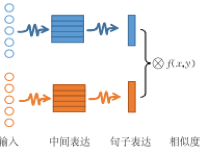
\includegraphics[width=1.0\linewidth]{match_single_doc.png}
  \caption{单文档语义表达匹配框架}{text match based on single document semantics}
  \label{fig:text match based on single document semantics}       % Give a unique label
\end{figure}

深度语义结构模型\cite{Huang2013LearningDS}是最早利用深度学习进行文本匹配的工作,主要是针对查询和文档的匹配任务。它通过搜索引擎里查询和文档的点击日志,利用深度网络得到查询和文档的向量表示,通过余弦相似度计算两个句子的语义相似度,最终得到相似度模型。

深度语义结构模型主要分成3层:输入、表示和匹配层。输入层上对于引文的处理方式为词哈希(word hashing),将每个英文单词切分成 3 个字母为一组的单词。这样可以压缩空间。增强泛化能力;中文以单字的一位有效编码(one-hot)进行输入。在表示层,采用词袋(Bag of words)的方式,输入一个 4 层神经网络,输出 128 维的向量表示,匹配层使用 softmax 进行分类预测。

\begin{figure}[!htbp]\centering
  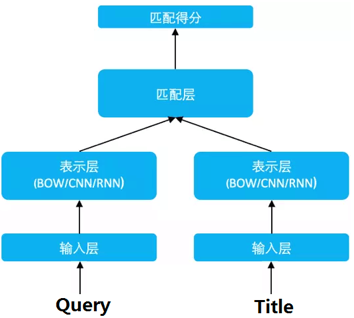
\includegraphics[width=1.0\linewidth]{DSSM.png}
  \caption{深度语义结构模型}{DSSM model}
  \label{fig:DSSM}       % Give a unique label
\end{figure}

图\ref{fig:DSSM} 表示了DSSM的网络结构,图中 $W_i,b_i$ 表示第 $i$ 层全连接的权重。DSSM 使用3个全连接层对文档语义进行建模,最后输出一个 128维的语义向量 $y$:

$$
\begin{aligned}
l_1 &= W_1x\\
l_i &= f(W_il_{i-1} + b_i), i=2,...,N-1\\
y &= f(w_Nl_{N-1} + b_N)
\end{aligned}
$$

我们使用tanh作为隐层和输出层的激活函数:
$$
f(x) = \frac{1-e^{-2x}}{1+e^{-2x}}
$$

最后利用 cosine 距离衡量两个语义向量的相似度:
$$
R(Q, D) = \text{cosine}(y_Q,y_D) = \frac{y_Q^Ty_D}{\|y_Q\|\|y_D\|}
$$
最后通过 softmax 函数将查询与正样本的相似度转化为概率分布:
$$
P(D^+|Q) = \frac{\exp\left(\gamma R(Q, D^+)\right)}{\sum_{D'\in D}\exp\left(\gamma R(Q, D')\right)}
$$
式中的 $\gamma$ 表示平滑因子,$D^+$表示匹配的正样本,其他句子均为负样本(负样本通过在整个文档空间随机采样获得),$D$ 表示整个文档空间。在训练时最小化损失函数

$$
\ell(\Lambda) = -\log \prod_{(Q,D^+)} P(D^+|Q)
$$

这种方法可以减少对切词算法的依赖,提高模型的泛化能力。但是由于使用词袋模型,丧失了语序信息和上下文信息,而且全连接的神经网络参数过多,难以训练。

针对于上面的问题,微软提出了基于单词序列的卷积深度语义模型(CLSM)\cite{Shen2014ALS}。与 DSSM 相比,CLSM 主要对输入和表示层进行了改进。
在输入层上,CLSM加入了一个滑动窗口,利用滑动窗口提取序列信息。

\begin{figure}[!htbp]\centering
  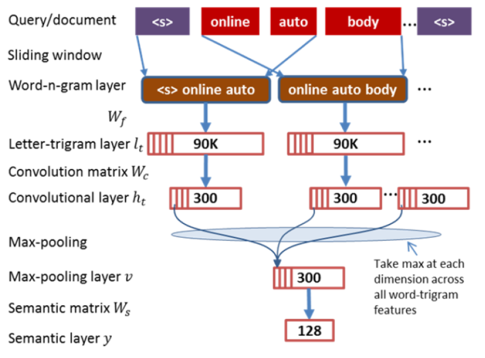
\includegraphics[width=1.0\linewidth]{CLSM.png}
  \caption{CLSM模型结构}{CLSM model}
  \label{fig:CLSM}       % Give a unique label
\end{figure}

在 \ref{fig:CLSM} 的结构中,我们可以看到选择的滑动窗口大小为3。对于一个滑动窗口内的词,类似DSSM,它将每个单词的3-字母组合的词哈希向量相加得到最终的向量表示。原模型中所使用的数据集最终被映射为 9 万维的向量。在表示层上,我们可以看到模型使用了卷积神经网络,利用卷积层的特征进行上下文的特征提取,利用池化层发现全局的上下文特征,最后利用全连接层将结果映射到一个128维的向量空间。这里的激活函数和DSSM相同,也采用了tanh。

在得到了 128 维的向量空间之后,CLSM 也采用了 cosine 距离计算两个语义向量的相似度,在概率分布的转化和损失函数上和 DSSM 都类似,因此不做过多描述。

\begin{figure}[!htbp]\centering
  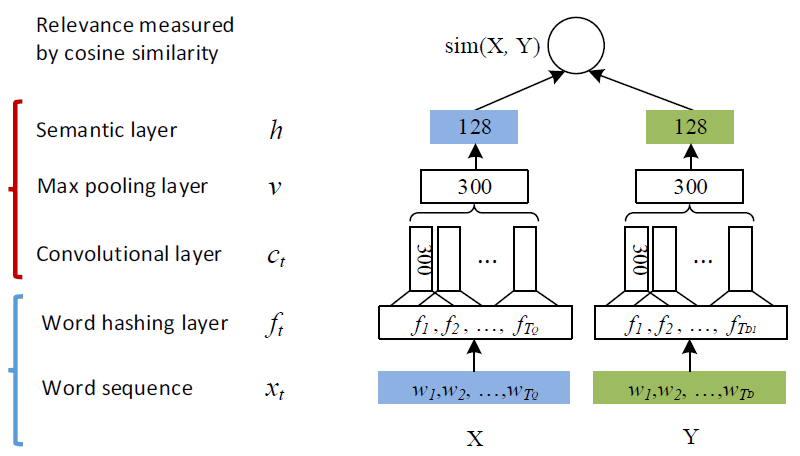
\includegraphics[width=0.8\linewidth]{CLSM_network}
  \caption{CLSM表示层网络结构}{Neural network struct of CLSM}
  \label{fig:CLSM_network}       % Give a unique label
\end{figure}

相对于DSSM,CLSM 通过卷积和池化提取全局的上下文信息,但是对于间隔较远的上下文信息,由于卷积神经网络的限制仍然难以捕捉。

针对于这种问题,有人想到利用 LSTM\cite{Hochreiter1997LongSM}(Long-Short-Term Memory)建模上下文信息,提出了LSTM-DSSM\cite{Palangi2014SemanticMW}。

LSTM是对 RNN(Recurrent Neural Networks) 的改进。RNN是一种用于处理序列信息的神经网络,在处理序列信息是,RNN中每个节点的权值是共享的。

\begin{figure}[!htbp]\centering
  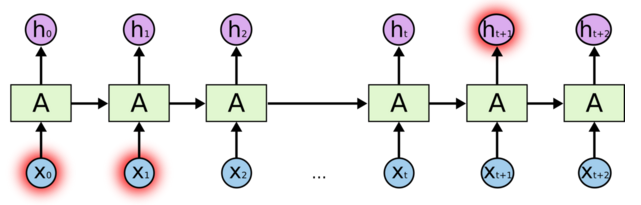
\includegraphics[width=0.8\linewidth]{RNN}
  \caption{RNN 网络结构}{Recurrent Neural Network}
  \label{fig:RNN}       % Give a unique label
\end{figure}

图\ref{fig:RNN} 描述了一个简单的 RNN 网络结构。图中每个节点A的权重都是共享的。但是由于RNN的网络跟序列长度有关,因此当RNN的序列长度过长时,梯度消失的情况会十分明显。这导致 RNN 难以对长序列建模。为了解决这个问题,有人提出了 LSTM:

\begin{figure}[!htbp]\centering
  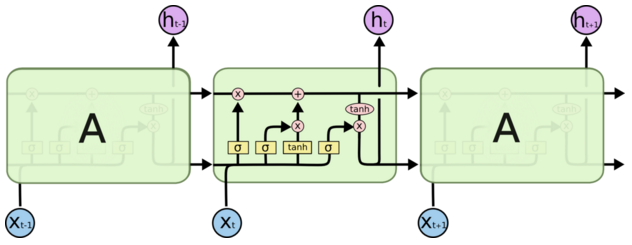
\includegraphics[width=0.8\linewidth]{LSTM}
  \caption{LSTM 网络结构}{Long-Short-Term Memory}
  \label{fig:LSTM}       % Give a unique label
\end{figure}

LSTM 利用遗忘门控制一个节点可以通过的信息量;利用输入们确定要添加到节点的数据;利用输出门确定输出的信息:
$$
\begin{aligned}
f_t&=\sigma(W_f[h_{t-1}, x_t] + b_f) \\
i_t&=\sigma(W_i[h_{t-1}, x_t] + b_i)\\
\tilde{C}_t &= \text{tanh}(W_C[h_{t-1}, x_t] + b_C)\\
o_t&=\sigma(W_o[h_{t-1}, x_t] + b_o)\\
h_t&=o_t\text{tanh}(\tilde{C}_t)
\end{aligned}
$$
通过这种方式,LSTM可以有效避免RNN网络的梯度消失问题。

LSTM-DSSM整体的网络结构为:

\begin{figure}[H]\centering
  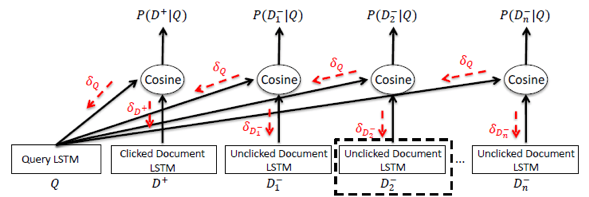
\includegraphics[width=0.8\linewidth]{LSTM-DSSM.png}
  \caption{LSTM-DSSM模型结构}{LSTM-DSSM model}
  \label{fig:LSTM-DSSM}       % Give a unique label
\end{figure}

相对于CLSM,LSTM-DSSM主要是将 CNN 换成了 LSTM。

DSSM本身是端到端的模型,虽然它省下了算法工程师特征工程部分的操作,但是其效果不可控;而且 DSSM 都是弱监督模型,需要大量的训练样本进行训练。在 DSSM论文中,作者提到实际训练所使用的样本量超过一亿,而且论文中所使用的样本都是曝光置信度较高的样本。这些限制因素极大的限制了 DSSM 的使用场景,往往只有少量大公司才可以使用。

这种情况下开始有学者关注于直接利用深度学习建模匹配的模型,提取句子之间的交互特征。这种方式更加直观,也更符合人类判断两个句子是否相似的过程。

MatchPyramid\cite{Pang2016TextMA}利用匹配矩阵建模两个句子的交互过程。匹配矩阵中每个值都是2个句子中词两两计算得到的相似度。相似度可以使用词向量的余弦相似度或点积等进行刻画,而2个词在各自句子中的位置自然组成了一个二维坐标,因此构造出了匹配矩阵。之后将匹配的问题建模为在这个矩阵上进行图像识别的过程,利用卷积和池化操作捕捉局部和全局的交互信息。

\begin{figure}[!htbp]\centering
  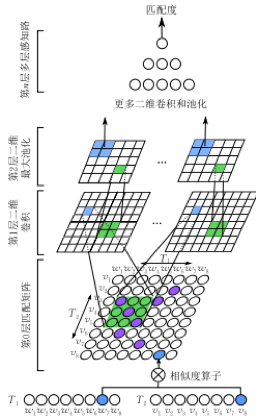
\includegraphics[width=0.4\linewidth]{MatchPramid.png}
  \caption{MatchPramid 模型}{MatchPramid model}
  \label{fig:MatchPramid}       % Give a unique label
\end{figure}

但是和CDSSM类似,利用 CNN 建模文本匹配的过程很可能失去文本的序列信息。因此有人提出了 MatchSRNN\cite{Wan2016MatchSRNNMT},利用 RNN 对匹配矩阵进行建模。但是 RNN 本身只能处理一维序列信息,因此 MatchSRNN 使用了Spatial RNN\cite{Graves2007MultidimensionalRN} 进行建模。Spatial RNN 的每个节点接受4个输入:
$$
\vec{h}_{ij} = f(\vec{h}_{i-1,j},\vec{h}_{i,j-1},\vec{h}_{i-1,j-1},\vec{s}_{ij})
$$
式中 $\vec{h}_{ij}$ 表示在匹配矩阵 $(i, j)$ 位置上的隐状态,$\vec{s}_{ij}$表示在匹配矩阵 $(i, j)$ 位置上的输入。MatchSRNN 使用了RNN的变种 GRU\cite{Cho2014LearningPR}(Gated Recurrent Unit)。 GRU 是对 LSTM 的简化,LSTM 中有三个门:遗忘门、输入门和输出门,GRU中只有两个门:更新门和重置门。更新门和重置门都控制历史状态对当前状态的影响,更新门控制了历史状态进入当前单元的程度,重置门控制了当前状态忽略历史状态。

\begin{figure}[!htbp]\centering
  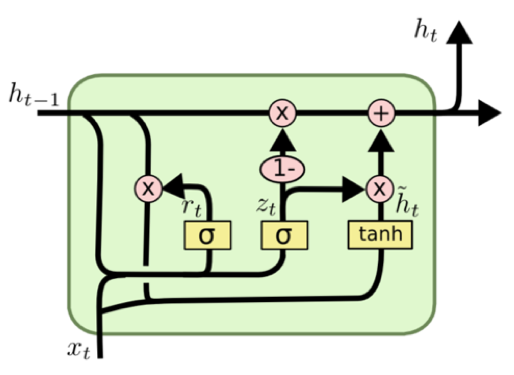
\includegraphics[width=0.8\linewidth]{GRU}
  \caption{GRU 模型}{Gated Recurrent Unitl}
  \label{fig:GRU}       % Give a unique label
\end{figure}

GRU 的计算方式为:
$$
\begin{aligned}
r_t &= \sigma(W_r[h_{t-1},x_t])\\
z_t &= \sigma(W_z[h_{t-1},x_t])\\
\tilde{h}_t &= \text{tanh}(W_{\tilde{h}}[r_t \times h_{t-1},x_t]) \\
h_t &= (1-z_t)\times h_{t-1} + z_t\times\tilde{h}_t
\end{aligned}
$$

Spatial GRU的计算方式为:
$$
\begin{aligned}
&\vec{q}^T = [\vec{h}^T_{i-1,j}, \vec{h}^T_{i-1,j-1}, \vec{h}^T_{i,j-1}, \vec{s}_{ij}^T]^T \\
&\vec{r}_l = \sigma(W^{(r_l)}\vec{q} + \vec{b}^{(r_l)})\\
&\vec{r}_t = \sigma(W^{(r_t)}\vec{q} + \vec{b}^{(r_t)})\\
&\vec{r}_d = \sigma(W^{(r_d)}\vec{q} + \vec{b}^{(r_d)})\\
&\vec{r}^T = [\vec{r}_l^T, \vec{r}_t^T, \vec{r}_d^T]^T\\
&\vec{z}'_i = W^{(z_i)}\vec{q} + \vec{b}^{(z_i)} \\
&\vec{z}'_l = W^{(z_l)}\vec{q} + \vec{b}^{(z_l)} \\
&\vec{z}'_t = W^{(z_t)}\vec{q} + \vec{b}^{(z_t)} \\
&\vec{z}'_d = W^{(z_d)}\vec{q} + \vec{b}^{(z_d)} \\
&[\vec{z}_i,\vec{z}_l,\vec{z}_t,\vec{z}_d] = \text{SoftmaxByRow}([\vec{z}'_i,\vec{z}'_l,\vec{z}'_t,\vec{z}'_d])\\
&\vec{h}'_{ij} = \phi(W\vec{s}_{ij} + U(\vec{r}\odot[\vec{h}^T_{i-1,j}, \vec{h}^T_{i-1,j-1}, \vec{h}^T_{i,j-1}]^T) + \vec{b})\\
&\vec{h}_{ij} = \vec{z}_l\odot\vec{h}_{i,j-1} + \vec{z}_t\odot\vec{h}_{i-1,j} + \vec{z}_d\odot\vec{h}_{i-1,j-1} + \vec{z}_i\odot\vec{h}'_{i,j}
\end{aligned}
$$
式中的 SoftmaxByRow 对每一个维度进行线性变换:

$$
[\vec{z}_p]_j = \frac{e^{[\vec{z'}_p]_j}}{e^{[\vec{z'}_i]_j}+e^{[\vec{z'}_l]_j}+e^{[\vec{z'}_t]_j}+e^{[\vec{z'}_d]_j}}, p=i,l,t,d
$$

MatchSRNN利用 Spatial GRU 对计算整个匹配矩阵,对Spatial GRU 进行全连接层进行非线性变换得到最后的结果。

\begin{figure}[!htbp]\centering
  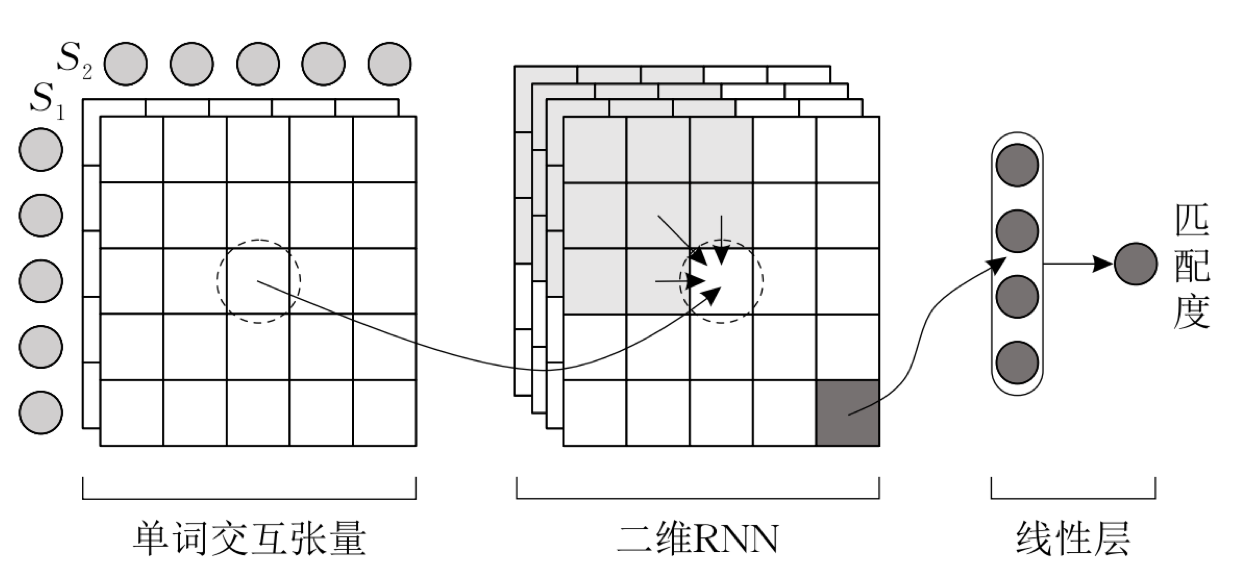
\includegraphics[width=0.8\linewidth]{MatchSRNN}
  \caption{MatchSRNN 模型}{MatchSRNN model}
  \label{fig:MatchSRNN}       % Give a unique label
\end{figure}

\section{强化学习研究现状}
\label{sec:rl_intro}
强化学习\cite{Sutton1998ReinforcementL}是机器学习中的一个重要研究领域,它以试错的机制与环境(Environment)进行交互,通过最大化累积奖赏来学习最优策略。强化学习研究的问题往往有三个特征:闭环性,学习系统产生的行为(action)会影响后续输出;无监督,学习对象只能通过学习得到行为的信息;行动产生的结果,包括奖励(reward),会影响较长时间。

一个强化学习过程可以被定义为一个五元组<$S, A, P, R, \pi$>,其中:
\begin{itemize}
  \item[•] 状态(Status,S)是环境的状态;
  \item[•] 动作(Action, A)是主体在特定环境下使用的策略
  \item[•] 转移概率(Transition function,P)是环境受主体动作影响后状态的迁移概率;
  \item[•] 奖励(Reward,R)是环境根据主体行为返回给主体的信号,主体根据奖励调整自己的策略;
  \item[•] 策略(Policy,$\pi$)定义了特定环境下主体的行为方式,表示状态到动作的映射关系。策略分为确定性和随机性两种。
\end{itemize}

\begin{figure}[!htbp]\centering
  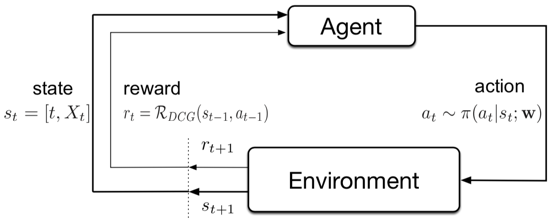
\includegraphics[width=1.0\linewidth]{interaction.png}
  \caption{主体与环境的交互}{interaction between agent and enviroment}
  \label{fig:interaction}       % Give a unique label
\end{figure}

主体和环境的交互可以用图\ref{fig:interaction}表示。主体在当前状态$s_t$下根据策略π选择动作$a_t$,环境接收到该动作并转移到下一状态$s_{t+1}$,主体接收环境反馈回来的奖励选择下一步动作。强化学习不需要监督信号,主要算法包括Q学习(Q-learning),策略梯度(policy gradient)等等。

深度强化学习的主要思路是将神经网络用于抽取复杂高维数据中的信息,并将其映射到一个低维向量空间便于强化学习处理。
由于卷积神经网络在计算机视觉领域的统治地位,DeepMind团队在2013年尝试将卷积神经网络和强化学习结合,提出来深度Q网络(DeepQ Network,DQN)\cite{Mnih2013PlayingAW},并成功的将该方法用在了Atari视频游戏。这是深度强化学习首次在高维度的状态空间下起作用。

2015年,DeepMind团队进一步完善了DQN算法\cite{Mnih2015HumanlevelCT}。
DQN将深度卷积神经网络和Q学习结合到一起,并集成了经验回放技术(memory reply)和目标Q网络。
经验回放通过随机采样系统在探索环境时得到的状态数据对神经网络参数进行更新,打破了Q-学习算法采样数据之间的相关性。DQN在没有任何人类先验知识的情况下在Atari视频游戏表现出了等同人类玩家的水平纪念,是深度强化学习领域的重要工作。

2016年初,DeepMind团队发表了围棋AI:AlphaGo\cite{Silver2016MasteringTG}。AlphaGo 利用强化学习指导蒙特卡罗树搜索的过程,将深度强化学习的研究推向了新的高度。它通过策略网络学习不同位置的落子概率,利用价值网络学习棋局的胜率评估,通过策略和价值网络的结合减小了蒙特卡罗树搜索的搜索次数,提高了搜索效率。在在线对弈时,利用蒙特卡罗树搜索以及策略和价值网确定当前的落子位置。

\begin{figure}[!htbp]\centering
  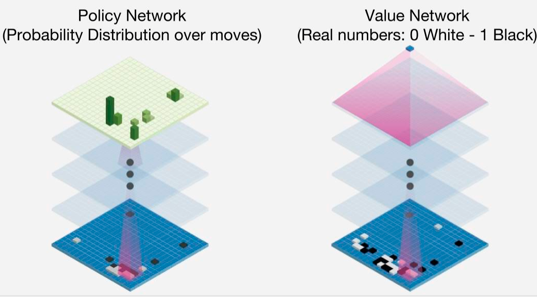
\includegraphics[width=0.8\linewidth]{AlphaGo.png}
  \caption{AlphaGo的策略网络和价值网络} {AlphaGo policy and value network}
  \label{fig:AlphaGo}       % Give a unique label
\end{figure}

2017年初,AlphaGo Zero\cite{Silver2017MasteringTG}对AlphaGo进行了改进和升级。AlphaGo Zero 抛弃了 AlphaGo 复杂的特征输入,只需要将棋局图片作为数据即可;将策略网络和价值网络整合在一起,直接利用深度强化学习方法进行端到端的自我对弈学习。
相比于 AlphaGo,AlphaGo Zero 去除了棋手的落子网络,因此不需要任何先验知识;策略网络和价值网络的整合使得神经网络的复杂度降低,泛化性进一步增强,降低了硬件的资源需求,减少了训练时间。

AlphaGo Zero的成功证明了在没有任何先验经验的情况下,深度强化学习在围棋领域仍然能取得巨大的成功;而在围棋下法上,AlphaGo Zero创造了更多的下棋方式,大大开拓了人类对围棋的认知。
虽然基于蒙特卡罗树搜索的深度强化学习方案已经取得了成功,但是由于搜索算法带来的时间和空间开销,使得其很难满足实时性的需求。目前强化学习很难在星际争霸这种实时游戏上战胜人类。

\begin{figure}[!htbp]\centering
  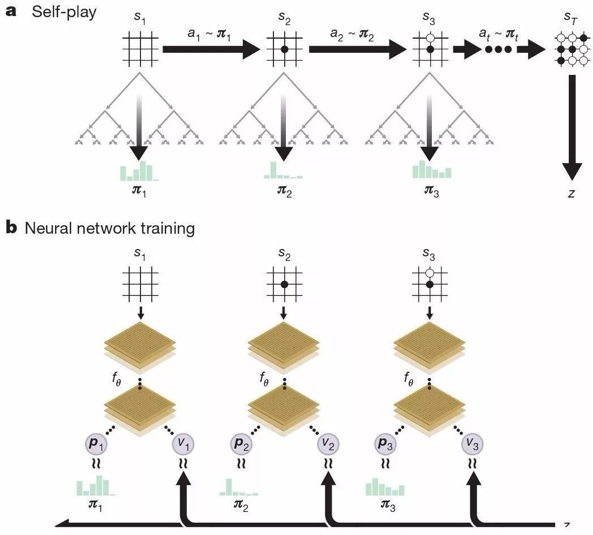
\includegraphics[width=0.8\linewidth]{AlphaGo_Zero.png}
  \caption{AlphaGo Zero 自我对弈训练过程} {training process of AlphaGo Zero}
  \label{fig:AlphaGo_Zero}       % Give a unique label
\end{figure}

\section{本章小结}

本章主要介绍了文本匹配和强化学习的相关工作与研究现状。

本章的第一小节主要介绍了基于深度学习的文本匹配算法。目前基于深度学习的文本匹配算法大都集中于利用神经网络理解输入句子的语义信息。最早利用深度学习解决文本匹配问题是DSSM。DSSM 利用词哈希以及词袋的方式得到句子的向量表示,并利用一个三层的全连接网络将句子的向量表示映射为一个低维向量表示。最后利用余弦相似度计算两个语义向量的距离,并利用 softmax 对得到的结果进行非线性变换,得到最后的概率分布。DSSM 通过词哈希降低了对且此算法的依赖,但是由于词袋模式的使用使其难以捕捉句子的上下文信息,而且全连接网络参数量极大,很难训练。为了解决 DSSM 模型问题,有人提出了CDSSM。相比于DSSM,CDSSM在词哈希的基础上引入了滑动窗口,通过滑动窗口解决了DSSM中上下文信息建模苦难的问题。同时 CDSSM 在表达网络中引入了卷积和池化操作,通过卷积建模上下文特征,利用池化发现全局特征,最后利用一个全连接层将结果映射到一个低维向量空间。但是由于卷积神经网络不是为序列化设置,因此对于长句子的上下文信息,CDSSN仍然难以捕捉。针对这个问题,有人提出将 LSTM 用于表达网络。DSSM及其后续的改进工作虽然有效的提高了文本匹配的效果,但是 DSSM 端到端的学习方式以及弱监督特征决定了它的利用场景十分有限。这种情况下有人提出了直接建模匹配模型的方法。MatchPyramid 利用两个句子之间词的相似度构造了一个匹配矩阵,将文本匹配过程视为对这个匹配矩阵的分类过程。 MatchPyramid 使用 CNN 建模了分类过程。和 MatchPyramid 类似, MatchSRNN 在匹配矩阵上使用了一个二维的 GRU 建模文本匹配的过程。

本章的第二小节主要介绍强化学习。强化学习是机器学习中的一个重要领域,最早用于机械控制领域,强调如何基于环境行动已获得最大收益。早期的增强学习方法包括策略梯度,值迭代等等,但是由于数据量过小,模型表达能力不强等等原因,强化学习的建模能力一直不强。近年来强化学习和深度学习的结合大大增加了强化学习的表达能力,使得强化学习近年来获得了长足的发展。DeepMind 提出了 DQN 并将其用于 Atari 游戏中,强化学习首次拥有了在高维状态空间下解决问题的能力。
16年初,DeepMind 团队提出了 AlphaGo 算法,该算法将强化学习和蒙特卡罗树搜索结合,通过策略网络和价值网络指导蒙特卡罗树搜索过程,大大提升了蒙特卡罗树搜索的速度。去年 DeepMind 进一步改进了 AlphaGo 算法,提出了 AlphaGo Zero。AlphaGo Zero 算法在没有任何人类先验知识的情况下在围棋领域取得了巨大的成功。

目前深度学习和强化学习的结合使得强化学习的表达能力大幅度上升,为学习传统文本匹配中复杂的规则和模式带来了可能。由于目前计算机理解人类语义十分困难,因此基于模式匹配的方式在短文本匹配场景中仍然拥有巨大的价值。本文会结合强化学习和文本匹配的特点,设计使用与文本匹配的强化学习算法。

\chapter{面向模式文本匹配的马尔科夫决策过程}

由于文本匹配的适用领域较为广泛,因此在各大互联网公司得到了大量的应用,创造了巨大的商业价值。基于强化学习的文本匹配可以较好的建模模式匹配中的规则。本文介绍了强化学习的主要技术,并且提出了模式文本匹配的算法设计。

\section{马尔科夫决策过程}
强化学习中,在某一时刻 $t$ ,主体会处于状态 $s_t$,并从环境中得到观测 $o_t$,根据观测和行动利用策略 $\pi_\theta(a_t|o_t)$ 或者 $\pi_\theta(a_t|s_t)$作出行动 $a_t$,环境根据主体状态 $s_t$ 以及行动 $a_t$ 通过转移概率分布函数 $p(s_{t+1}| s_t, a_t)$ 得到状态 $s_{t+1}$,通过奖励函数 $r(s, a)$ 得到奖励 $r_t$,周而复始。强化学习的目标即最大化总收益。

\begin{figure}[!htbp]
    \centering
    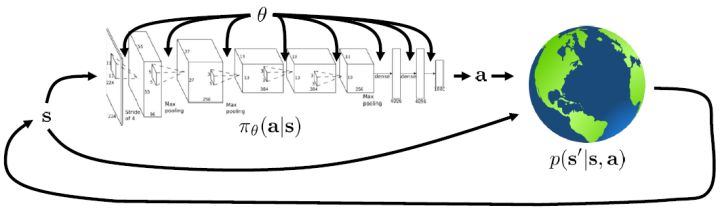
\includegraphics[width=1.0\textwidth]{MDP}
    \bicaption{马尔科夫决策过程}{Markov Decision Process}
    \label{fig:MDP}
\end{figure}

状态 $s$,行动 $a$,奖励函数 $r(s,a)$ 以及转移概率 $p(s'|s,a)$ 定义了马尔科夫决策过程。

在描述马尔科夫决策过程前,先简要介绍马尔科夫链。马尔科夫链 $M=\{S, P\}$ 由状态空间 $S$ 和转移概率 $P$ 组成。其中状态 $s$既可以是离散的变量,也可以是连续的数值;转移概率$p(s_{t+1}|s_t)$ 确定了在当前状态下转移到下一个状态的概率。令转移概率 $P_{i, j}=p(s_{t+1}=i|s_t=j)$,则这些概率组成了概率转移矩阵 $\mathcal{P}$。马尔科夫链具有马尔科夫性,即转移概率只与当前的状态有关。

马尔科夫过程是马尔科夫链在决策环境中的扩展 $M=\{S, A, P, R, \pi\}$。其中状态空间 $S$ 与马尔科夫链类似;行动空间 $A$ 即行动的集合;转移概率 $P$ 不仅受到当前状态的影响,还受到行动 $a\in A$ 的影响;$R$ 为奖励函数,是一个 $S\times A\to \mathbb{R}$ 的映射;策略 $\pi$ 表示在当前状态下每个行为的概率。

强化学习的过程中 $S, A, P, R$ 都是环境确定的,我们需要学习 $\pi(a|s)$ 以最大化长期收益。$\pi(a|s)$  可以由一个参数为 $\theta$ 的模型确定,记为 $\pi_\theta(a|s)$。

考虑一个有限长度的轨迹 $\tau=\{s_1,a_1,...s_t,a_t\}$,它产生的概率
$$
p_\theta(\tau) = p(s_1)\prod_{t=1}^T \pi_\theta(a_t|s_t)p(s_{t+1}|s_t,a_t)
$$
初始状态 $s_1$ 往往是确定的。根据马尔科夫性,后面每个时刻的行动和状态都是由当前的行动确定的。我们希望优化
$$\theta^* = \arg\max_\theta E_{\tau\sim p_\theta(\tau)}[\sum_t r(s_t, a_t)]$$以最大化总收益函数关于轨迹的期望。

对于有限长度的轨迹,我们在求解 $\theta^*$ 时只需要关注马尔科夫链在一个时间点上的边际分布;对于无限长度的轨迹,根据马尔科夫性,有
$$\left[\begin{array}{l}\mathbf{s}_{t+k}\\\mathbf{a}_{t+k}\end{array}\right]=\mathcal{P}\left[\begin{array}{l}\mathbf{s}_{t+k-1}\\\mathbf{a}_{t+k-1}\end{array}\right]=...=\mathcal{P}^k\left[\begin{array}{l}\mathbf{s}_{t}\\\mathbf{a}_{t}\end{array}\right]$$
对于无限长度的问题,当到达平稳分布时,我们可以对目标进行平均:
$$
\theta^*=\arg\max_\theta\frac{1}{T}\sum_{t=1}^T\mathbf{E}_{(\mathbf{s}_t,\mathbf{a}_t)\sim p_\theta(\mathbf{s}_t,\mathbf{a}_t)}r(\mathbf{s}_t,\mathbf{a}_t)\rightarrow \mathbf{E}_{(\mathbf{s},\mathbf{a})\sim p_\theta(\mathbf{s},\mathbf{a})}r(\mathbf{s},\mathbf{a})
$$

一个完整的强化学习的训练过程一般包含 3 个部分:

1. 生成样本。在模拟器中运行我们当前的策略并收集轨迹(trajectory)样本。轨迹的收集即主体和环境的交互过程:在 $t$ 时刻,我们从环境得到观测信息 $o_t$,在此观测信息下根据策略 $\pi_\theta(a_t|o_t)$ 得到当前的行动 $a_t$,根据系统的转移概率 $p(s_{t+1}|s_t, a_t)$ 得到下一个状态 $s_{t+1}$。在做出当前的行动之后,我们会得到收益 $r(s_t,a_t)$, 简记为 $r_t$ 。我们的目标就是最大化得到的总收益。

2. 收益估计。不同的算法在这一步的表现不尽相同。对于策略学习来说,就是策略评估;对于基于模型的增强学习算法,就是模型拟合。

3. 改进策略。根据上一步得到的结果改进策略,再执行第一步,循环往复。

\begin{figure}[!htbp]
    \centering
    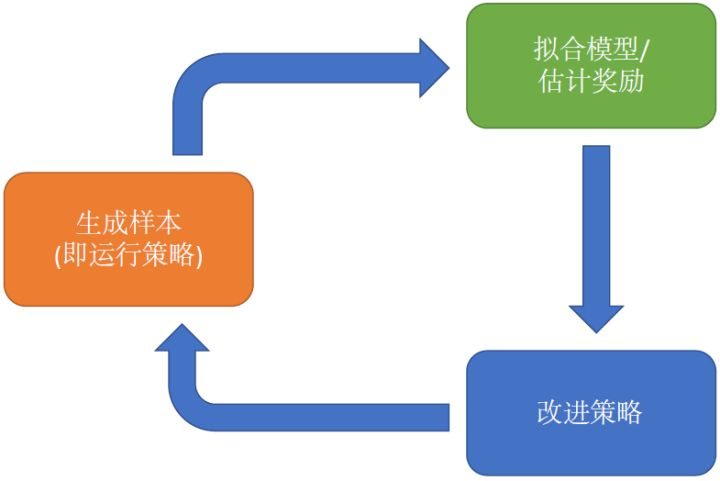
\includegraphics[width=0.7\textwidth]{RL_process}
    \bicaption{增强学习算法的一般步骤}{Reinforcement Learning Process}
    \label{fig:RL_process}
\end{figure}

\subsection{马尔科夫决策过程求解}

但是由于强化学习中在样本生成时得到的行动以及系统的状态转移都带有一定的随机性,因此我们希望最大化奖励的条件期望
\begin{equation}\label{eq:max_expect}
G_t = R_{t+1} + \gamma R_{t+2} + ... = \sum_{k=0}^\infty \gamma^kR_{t+k+1}
\end{equation}
$\gamma$ 表示折现率。

我们将值函数(value fuction)定义为一个状态在未来的价值,即回报的期望。那么值函数可以被表示为:
\begin{equation}\label{eq:Bellman}
\begin{aligned}
v(s) & = E[G_t|S_t = s] \\
     & = E[R_{t+1} + \gamma R_{t+2} + \gamma^2 R_{t+3}+...|S_t=s]\\
     & = E[R_{t+1} + \gamma(R_{t+2} + \gamma R_{t+3}+...)|S_t=s]\\
     & = E[R_{t+1} + \gamma G_{t+1}|S_t=s]\\
     & = E[R_{t+1} + \gamma v(S_{t+1})|S_t=s]\\
\end{aligned}
\end{equation}

\eqref{eq:Bellman} 被称为 Bellman 方程,它表明 value function 可以通过迭代计算得到。我们的目的就是通过迭代优化最大化 $v(s)$

通过 Bellman 方程,我们可以得到:
\begin{equation}
\begin{aligned}
v_{k+1}(s) & = E[R_{t+1} + \gamma v_k(S_{t+1})|S_t=s]\\
           & = \sum_a \pi(a|s)\sum_{s',r}p(s', r| s, a)[r+\gamma v_k(s')]
\end{aligned}
\end{equation}
我们可以通过迭代计算价值函数来优化策略收敛到最优。

策略迭代一般分成两步:策略评估和策略改进。利用当前策略产生新样本,使用新样本更新当前策略,最终收敛到最优。在策略评估时需要知道环境的状态转移概率,因此策略迭代需要依赖模型。

\begin{algorithm}[H]
    \small
    \caption{policy iteration}\label{alg:policy_iteration}
    \begin{algorithmic}
        \State Step 1. Initialization
        \State $V(s) \in \mathbb{R}$ and $\pi(s) \in \mathcal{A}(s)$ aribitrarily for all $s \in \mathcal{S}$
        \State Step 2. Policy Evaluation
        \Repeat
        \State $\Delta \leftarrow 0$
        \For {each $s \in \mathcal{S}$}
        \State $v \leftarrow V(s)$
        \State $V(s)\leftarrow \sum_{s', r} p(s', r|s, \pi(s))[r + \gamma V(s')]$
        \State $\Delta \leftarrow \max(\Delta, |v-V(s)|$
        \EndFor

        \Until{$\Delta < \theta$}

        \State Step 3. Policy Improvement
        \State policy-stable $\leftarrow  true$
        \For {each $s \in \mathcal{S}$}
        \State $a \leftarrow \pi(s)$
        \State $\pi(s) \leftarrow \arg\max_a\sum_{s', r}p(s', r|s, \pi(s))[r + \gamma V(s')]$
        \State If $a \neq \pi(s)$ then policy-stable $\leftarrow  false$
        \EndFor
        \State If policy-stable, then stop and return V and $\pi$; else go to 2
    \end{algorithmic}
\end{algorithm}

但是策略迭代算法每次都要进行策略评估和改进,这大大增加了算法的训练时间。由于对策略的改进和对值函数的改进是一致的,所以我们可以将策略改进视为对值函数的改进。

通过 Bellman 方程,我们可以得到:
\begin{equation}\label{eq:Bellman_value}
\begin{aligned}
v_{*}(s) & = E[R_{t+1} + \gamma v_*(S_{t+1})|S_t=s, A_t=a]\\
         & = \max_a \sum_{s',r}p(s', r| s, a)[r+\gamma v_k(s')]
\end{aligned}
\end{equation}

从 \eqref{eq:Bellman_value} 可以发现,我们可以通过 Bellman 最优模型来更新值函数收敛,最后收敛可以得到当前策略的最优值 $v_*$

\begin{algorithm}[!htbp]
    \small
    \caption{value iteration}\label{alg:value_iteration}
    \begin{algorithmic}
        \State Initialization array $V$ aribitrarily
        \Repeat
        \State $\Delta \leftarrow 0$
        \For {each $s \in \mathcal{S}$}
        \State $v \leftarrow V(s)$
        \State $V(s)\leftarrow \max_a\sum_{s', r} p(s', r|s, a)[r + \gamma V(s')]$
        \State $\Delta \leftarrow max(\Delta, |v-V(s)|$
        \EndFor
        \Until{$\Delta < \theta$}

        \State Output a deterministic policy, $\pi$ such that
        \State $\pi(s) = \arg\max_a\sum_{s', r} p(s', r|s, a)[r + \gamma V(s')]$
    \end{algorithmic}
\end{algorithm}

相比于 \ref{alg:policy_iteration},值迭代算法避免了策略评估部分的计算量,降低了算法运行时间,有效地提高了算法的运行效率。

我们发现无论是算法 \ref{alg:policy_iteration} 还是 \ref{alg:value_iteration},算法每次都是选择概率或者是值最高的行动。这种策略被称为利用(exploitation)。与之相对应的,如果我们每次都根据概率或者是值的分布进行采样,根据采样的结果采取行动,这种策略被称为探索(exploration)。探索的优势在于当信息匮乏是可以取得较好的效果,但是效率很低;利用的优势在于效率很高,但是只有在信息足够充足的情况下才会有效。

将探索和利用结合的算法被称为 $\epsilon$-贪心算法。我们在每次选择行动的时候,都以 $\epsilon$ 的概率进行探索,以 $1-\epsilon$ 的结果进行利用好。可以通过 $\epsilon$ 的调整在算法的不同阶段达到不同的效果。

\section{文本匹配的MDP介绍}
\label{sec:TM_MDP}
本节将文本匹配过程建模为一个强化学习过程。

在\ref{sec:text_matching} 节中,我们介绍了MatchSRNN\cite{Wan2016MatchSRNNMT} 算法。MatchSRNN 使用匹配矩阵中提取句子间的交互信息,利用二维 GRU 提取单个句子和句子之间的序列信息。 在二维 GRU计算完成后,通过二维 GRU 的状态,我们可以回溯出一条路径。
图\ref{fig:LD_dis}表示了对 $Q$=How to get rid of memory stick error of my
sony cyber shot?, $D$=You might want to try to format the memory
stick but what is the error message you are receiving. 得到的匹配矩阵进行回溯得到的路径。

\begin{figure}[H]
    \centering
    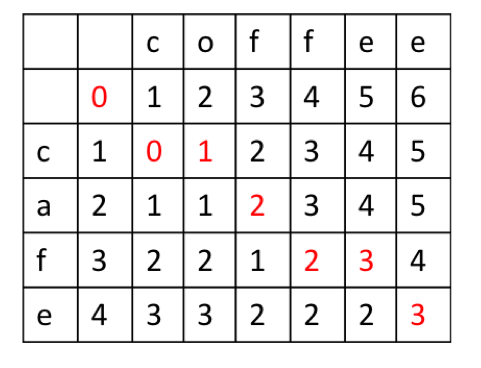
\includegraphics[width=0.60\textwidth]{LD_dis}
    \bicaption{MatchSRNN 的回溯路径}{Backtracing path of MatchSRNN}
    \label{fig:LD_dis}
\end{figure}

既然MatchSRNN通过回溯可以得到一条路径,那么一个直接的想法就是不通过二维GRU的方式直接获得一条路径,利用这条路径判断两个句子是否匹配。

\begin{figure}[!htbp]
    \centering
    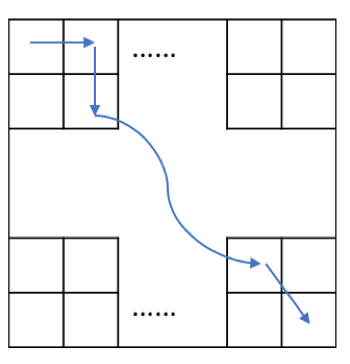
\includegraphics[width=0.40\textwidth]{match_MDP}
    \bicaption{文本匹配路径计算过程}{Pattern Text Matching}
    \label{fig:match_MDP}
\end{figure}

和 MatchPyramid 以及 MatchSRNN 类似,我们同样会使用匹配矩阵的概念。我们从匹配矩阵的右上角出发,根据当前位置确定行走方向,直到走到左下角为止。这样情况下我们会得到一条匹配路径。我们需要建立一个判别模型,根据匹配路径判断是否匹配。

首先描述文本匹配算法中获得匹配路径的过程,该过程为一个马尔科夫决策过程。其输入为一个句子对 $Q=\{\mathbf{u}_1, \mathbf{u}_2,\cdots,\mathbf{u}_n\}, D=\{\mathbf{v}_1, \mathbf{v}_2,\cdots,\mathbf{v}_m\}$

1. 状态 $\mathcal{S}$:我们将在 $t$ 时刻的状态 $s_t$ 定义为从当前位置开始向前看的 $m$ 个单词:
$$
\begin{aligned}
s_t &= \{[\mathbf{u}_{q_t}, \mathbf{v}_{d_t}], [\mathbf{u}_{1+q_t},\mathbf{v}_{1+d_t}] \cdots, [\mathbf{u}_{m+q_t}, \mathbf{v}_{m+d_t}]\}
\end{aligned}
$$
式中 $q_t$ 和 $d_t$ 表示当前位置。

2. 动作$\mathcal{A}$:在每个时间 $t$,我们都可以选择向下,向右或者像右下方行走。

3. 状态转移函数$\mathcal{T}(S,\mathcal{A})$:状态转移函数 $\mathcal{T}:S\times \mathcal{A}\rightarrow S$ 被定义为:
$$
(q_{t+1}, d_{t+1}) =
\begin{cases}
(q_{t} + 1, d_{t}) &\text{if goes down} \\
(q_{t}, d_{t} + 1) &\text{if goes right}  \\
(q_{t} + 1, d_{t} + 1) &\text{if goes obliquely}
\end{cases} \\
$$
$$
\begin{aligned}
s_{t+1} &= \mathcal{T}(s_t, a_t) = [\mathbf{u}_{q_{t+1}}, \mathbf{v}_{d_{t+1}}], [\mathbf{u}_{1+q_{t+1}},\mathbf{v}_{1+d_{t+1}}] \cdots, [\mathbf{u}_{m+q_{t+1}}, \mathbf{v}_{m+d_{t+1}}]
\end{aligned}
$$
在每个时间 $t$:系统根据当前的状态选择一个行动(移动方向),并根据方向移动到下一个位置,状态随之转移:根据当前的位置 $(q_{t+1}, d_{t+1}) $更新未来单词序列。完成转移后,再根据当前状态继续移动。

4.值函数 $V$:值函数 $V: S\rightarrow \mathbb{R}$ 是对当前模型是否可以得到正确预测结果的预测。值函数需要不断更新以更加准确的得到预测结果。本节所提出的值函数目的是预测模型是否可以预测成功,即 $\mathbf{1}_{t=y}$,其中 $t$ 为预测的 label, $y$ 为实际label。 值函数以两个句子当前位置的前 $m$ 个单词作为输入,确定当前句子是否可以正确判别。
我们利用一个 LSTM 网络处理输入的序列,通过对 LSTM 网络输出的加权和进行线性变换得到值函数:
$$
V(s) = \sigma(<w, g(s)>, b_v)
$$

其中 $g(s)$ 是LSTM网络的输出:

$$
g(s) = LSTM(Q[q_{t}:m+q_{t}], D [d_{t}:m+d_{t}])
$$

LSTM 网络接受两个长度为 $m$ 的单词序列,计算得到隐状态:

\begin{equation}
\label{eq:LSTM}
\begin{aligned}
f_k &= \sigma(W_f[Q_{k+q_{t}}, D_{k+d_{t}}] + U_fh_{k-1} + b_f) \\
i_k &= \sigma(W_i[Q_{k+q_{t}}, D_{k+d_{t}}] + U_ih_{k-1} + b_i) \\
o_k &= \sigma(W_o[Q_{k+q_{t}}, D_{k+d_{t}}] + U_oh_{k-1} + b_o) \\
c_k &= f_k \circ c_{K-1} + i_k \circ (W_c[Q_{k+q_{t}}, D_{k+d_{t}}] + U_ch_{k-1}+b_c) \\
h_k &= o_k \circ \text{tanh}(c_k)
\end{aligned}
\end{equation}

\begin{figure}[!htbp]
    \centering
    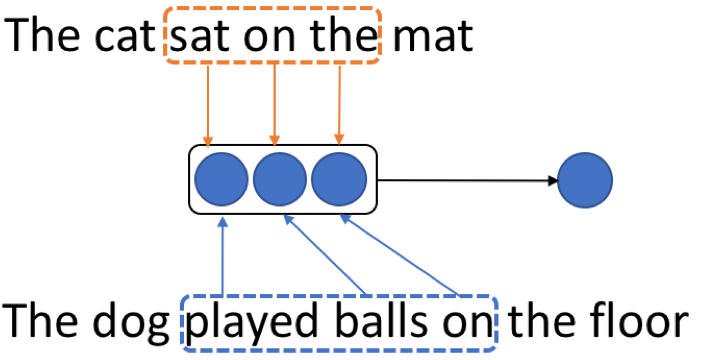
\includegraphics[width=0.80\textwidth]{match_value_function}
    \bicaption{文本匹配值函数输入}{value function input of text matching}
    \label{fig:value_function_input}
\end{figure}

图 \ref{fig:value_function_input} 以 $Q=\{\text{The cat sat on the mat}\},D=\{\text{The dog played balls on the floor}\}, m=3$ 为例展示了值函数。当前的状态 $s=[2, 2]$ ,我们将 $Q[2:5]=\{\text{sat, on, the}\}, D[2:5]=\{\text{played, balls, on}\}$ 的词向量作为 LSTM 的输入,利用 LSTM 捕捉未来词汇的序列信息,计算每个行为的值。

获得匹配路径的算法可以被表示为:
\begin{algorithm}[!htbp]
    \small
    \caption{MDP of Text Match}\label{alg:MDP_TM}
    \renewcommand{\algorithmicrequire}{\textbf{Input:}}
    \renewcommand{\algorithmicensure}{\textbf{Output:}}
    \begin{algorithmic}
        \Require Labeled data $D=\{ (\mathbf{Q}, \mathbf{D}, \mathbf{Y}) \}$
        \Ensure Path
        \State \text{Initialize} Path $\leftarrow [0, 0]$
        \State {set $q_1=0, d_2=0$}
        \While {$q_t < \text{len}(\mathbf{s}_1)$ and $d_t < \text{len}(\mathbf{s}_2)$}
        \State $a_t = \arg\max_a v(Q [q_t:m+q_t], D [d_t:m+d_t], a)$
        \State update status according to Eq \ref{eq:status_transfer}
        \State Path $\leftarrow$ Path $\oplus [q_t, d_t]$ \Comment{$\oplus$ means appends to end}
        \EndWhile
    \end{algorithmic}
\end{algorithm}

在计算路径时,算法从初始状态 $s_1 = [Q[1:m], D[1:m]]$ 出发,每次将当前位置的前 $m$ 个词作为输入,得到每个行动的值,选择值最大的行动作为当前的行动,并根据当前的行为移动到下一个位置,直到到达矩阵的右下角。一直选择值最大的行动可能会导致算法陷入局部最优解,因此可以采用 $\epsilon$-贪心的方法控制探索和利用的程度。

\subsection{匹配路径的判别}
\label{sec:path_classify}

在计算匹配路径之后,我们需要根据路径判断两个句子是否匹配。判别算法以原句子 $Q, D$ 以及对应的路径映射 $m_1 = [q_1, q_2, \cdots, q_t], m_2 = [d_1, d_2, \cdots, d_t]$ 作为输入,判断两个句子是否匹配。

我们利用3个LSTM网络作为判别模型,其中 LSTM$_1$ 和 LSTM$_2$ 将 $S_1$ 和 $S_2$ 映射为2个矩阵,LSTM$_c$ 将这两个矩阵映射为一个一维向量 $g_c(s)$:
$$
\begin{aligned}
f(Q) &= \text{LSTM}_1(Q) \\
h(D) &= \text{LSTM}_2(D) \\
g_c(s) &= \text{LSTM}_c([{f(Q)}_{q_1}, {h(D)}_{d_1}], [{f(Q)}_{q_2}, {h(D)}_{d_2}], \cdots, [{f(Q)}_{q_t}, {h(D)}_{d_t}])
\end{aligned}
$$

通过对 $g_c(s)$ 的加权和进行归一化得到最终的匹配概率
\begin{equation}
\label{eq:TM_classfiy}
p = \sigma(<w, g_c(s)> + b)
\end{equation}

其中 $w$ 和 $b$ 都是需要学习的参数,$\sigma(x) = \frac{1}{1+e^{-x}}$
LSTM 网络和 \ref{eq:LSTM} 类似, LSTM$_1$  和 LSTM$_2$ 共享参数。

\begin{figure}[!htbp]
    \centering
    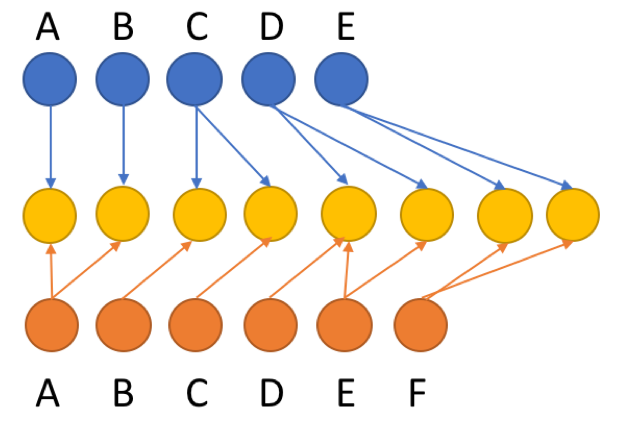
\includegraphics[width=0.40\textwidth]{path_classify}
    \bicaption{匹配路径判定}{match path classfiy}
    \label{fig:path_classify}
\end{figure}

\section{文本匹配 MDP 的训练与预测}
上节引入了文本匹配的 MDP,本节主要介绍文本匹配的MDP的训练与预测过程。我们利用值函数法进行文本匹配 MDP 的训练与预测,将我们的方法称为VIM(value iteration match)。
\subsection{训练过程}
训练时我们使用算法 \ref{alg:value_iteration} 进行优化。模型的参数包含 MDP 过程的参数 $\Theta_{MDP}$ 以及判别模型的参数 $\Theta_{c}$,在训练时,模型接受数据集 $D=\{Q^{(n)}, D^{(n)}, Y^{(n)}\}_{n=1}^N$ 作为输入,输出参数 $\Theta_{MDP}$ 以及 $\Theta_{c}$.

在训练阶段,每次迭代时,利用算法 \ref{alg:MDP_TM} 为每个样本$Q, D$生成一条路径

$$\{[q_1, d_1], [q_2, d_2], \cdots, [q_t, d_t]\}$$

并根据生成的路径以及真实结果训练路径判别模型。训练路径匹配模型时的损失函数为交叉熵:
\begin{equation}
\label{eq:classify_model}
\ell_c(Y, p) = -(Y\log(p) + (1-Y)\log(1-p))
\end{equation}

在路径判别模型收敛后,利用判别模型输出该路径为匹配的概率 $p$, 并利用 $p$ 计算奖励:
$$
r = \log(\frac{1}{|p-Y+\Delta|})
$$
其中 $\Delta$ 表示一个极小值以保证 $|p-Y+\Delta| > 0$.

之后我们利用$r$更新 $\Theta_{MDP}$。 MDP 过程的损失函数为:
\begin{equation}
\label{eq:MDP_model}
\ell(V(s), r) = \sum_{i=1}^t\left((y - V(r_i))^2\right)
\end{equation}

\begin{algorithm}[!htbp]
    \small
    \caption{Train Process of VIM}\label{alg:TM_train}
    \renewcommand{\algorithmicrequire}{\textbf{Input:}}
    \renewcommand{\algorithmicensure}{\textbf{Output:}}
    \begin{algorithmic}
        \Require Labeled data $D=\{ (\mathbf{Q}^{(n)}, \mathbf{D}^{(n)}, \mathbf{Y}^{(n)})\}_{n=1}^N$, learning rate $\eta$
        \Ensure $\Theta_{MDP}, \Theta_{c}$
        \State \text{Initialize} $\Theta_{MDP}, \Theta_{c} \leftarrow$ random values in $[-1, 1]$
        \While {not convergency}
          \State generate path according to Alg~\ref{alg:MDP_TM}
          \While {not convergency}
            \State $\Theta_{c} = \Theta_{c} - \eta \frac{\delta \ell_c}{\delta \Theta_{c}}$ \Comment{$\ell_c$ is defined in Eq~\ref{eq:classify_model}}
          \EndWhile
          \State $\Theta_{MDP} = \Theta_{MDP} - \eta \frac{\delta \ell}{\delta \Theta_{MDP}}$ \Comment{$\ell$ is defined in Eq~\ref{eq:MDP_model}}
        \EndWhile
    \end{algorithmic}
\end{algorithm}

\subsection{推断过程}
推断时,模型接收句子对 $Q, D$ 以及算法 \ref{alg:TM_train} 中得到的值函数 $V$ 作为输入,输出预测结果 $Y$。

在推断时,利用算法\ref{alg:MDP_TM} 为样本$Q, D$生成一条路径

$$\{[q_1, d_1], [q_2, d_2], \cdots, [q_t, d_t]\}$$

并将生成的路径输入到路径判别模型中,利用公式~\ref{eq:TM_classfiy} 计算得到最终的匹配概率。

\begin{algorithm}[!htbp]
    \small
    \caption{Inference Process of VIM}\label{alg:TM_inf}
    \renewcommand{\algorithmicrequire}{\textbf{Input:}}
    \renewcommand{\algorithmicensure}{\textbf{Output:}}
    \begin{algorithmic}
        \Require sentence pair $D=\{ (\mathbf{Q}^{(n)}, \mathbf{D}^{(n)})\}_{n=1}^N$, value function $V$
        \Ensure label $\mathbf{Y}$
        \State $s \leftarrow [1,1]$
        \State generate path according to Alg~\ref{alg:MDP_TM}
        \State compute $Y$ by Eq.~\ref{eq:TM_classfiy}
        \State \Return  $Y$
    \end{algorithmic}
\end{algorithm}

\section{实验与结果分析}
\subsection{实验数据}
为了对我们提出的文本匹配 MDP 的有效性进行评估,我们利用 Quora 的问题匹配数据集进行了测试。 Quora 是美国的在线知识问答平台,每天会产生大量的相似问题。该数据集即为 Quora 从其问答平台上收集到并进行了人工标注的匹配问题数据。

该数据集共包含约40万数据集,句子长度从3到100不等,能够较好的对模型的有效性进行评估。由于该数据集的样本量过大,我们从样本中挑选出了长度在 8到10 的约6万个句子对作为数据集,选择其中的 45056 个句子对作为训练集,22528个句子对作为验证集,4441个句子作为测试集对我们的算法进行了测试。

\subsection{评价准则}
为了比较不同算法的预测结果,本小节介绍用于文本匹配算法的评价准则。对于测试集 $S = \{S_1^{(n)}, S_2^{(n)}, Y^{(n)}\}_{n=1}^N$,文本采用的评价准则如下所述:

\begin{itemize}
  \item[•] 准确率: 计算<句子对,标签> 被正确划分的次数占总样本的比重。 $\text{acc}(S)$ 越大,算法在该准则上的表现越好;当 $\text{acc}(S) = 1$ 时,该评价指标达到最优值。
  $$
  \text{acc}(S) = \frac{\sum_i^N\mathbb{I}_{y_i=t_i}}{N}
  $$
  其中 $y_i$ 表示第 $i$ 个样本的预测结果, $t_i$ 表示第 $i$ 个样本的实际结果。
  \item[•] F1:对 <句子对,标签> 正样本准确率以及负样本准确率的调和平均值。 $\text{F1}(S)$ 越大,算法在该准则上的表现越好;当 $\text{F1}(S) = 1$ 时,该评价指标达到最优值。
  $$
  \begin{aligned}
  \text{P}(S) &= \frac{\sum_i^N\mathbb{I}_{y_i=t_i \text{and} t_i = 1}}{\sum_i^N\mathbb{I}_{t_i = 1}}\\
  \text{R}(S) &= \frac{\sum_i^N\mathbb{I}_{y_i=t_i \text{and} t_i = 0}}{\sum_i^N\mathbb{I}_{t_i = 0}}\\
  \text{F1}(S) &= \frac{2*P*R}{P+R}
  \end{aligned}
  $$
  \item[•] auc:ROC(Receiver Operating Characteristic) 曲线和坐标轴相交部分覆盖的面积大小。 ROC 曲线由两个变量 1-specificity 和 Sensitivity 绘制,分别反映了负样本和正样本的分类准确率。$\text{auc}(S)$ 越大,算法在该准则上的表现越好;当 $\text{auc}(S) = 1$ 时,该评价指标达到最优值。
\end{itemize}

\subsection{实验结果}
\label{sec:lab_value}
对于文本匹配问题,目前已经有多种算法可以很好地解决该问题。本文选取了其中两个经典的文本匹配算法 MatchPyramid\cite{Pang2016TextMA} 以及 MatchSRNN\cite{Wan2016MatchSRNNMT} 来与本文提出的算法进行比较。

在 Quora 数据集上。本文进行了算法的五折交叉验证。即将原始数据集合分割成五份,每份大小相同。每一折实验选择其中的四份数据作为训练集,一份数据作为验证集。上述过程重复五次,即每份数据都被用做验证集。每一折实验都选取验证集上评价准则最高的参数进行测试,将测试结果取平均值作为最后的评估结果。

\begin{table}[!htbp]
    \bicaption{文本匹配算法在 Quora 数据集上的测试结果}{The result of text matching algorithm on Quora dataset}
    \label{tab:MDP_test}
    \centering
    \footnotesize% fontsize
    \setlength{\tabcolsep}{4pt}% column separation
    \renewcommand{\arraystretch}{1.2}%row space
    \begin{tabular}{cccc}
        \hline
        \multirow{2}{*}{Algorithm} &
        \multicolumn{3}{c}{\multirow{1}{*}{Evaluation Criterion}} \\
        \cline{2-4} & acc & F1 & auc \\
        \hline
        VIM & $\textbf{0.7222}(*)$ & $0.7217$ & $\textbf{0.7979}(*)$ \\
        MatchPyramid & $0.7130$ & $\textbf{0.7220}(*)$ & $0.7853$ \\
        MatchSRNN & $0.7105$ & $0.7201$ & $0.7848$\\
        \hline
    \end{tabular}
\end{table}

可以发现 VIM 在 acc 和 auc 上均显著优于 MatchPyramid 和 MatchSRNN, 在 F1 上三者相差并不大。

根据在 QuoraQP 上的测试结果来看,使用值迭代的方式训练马尔科夫决策过程的收敛速度很快,图\ref{fig:value_iter_line}为我们的算法在上面试验中某一折数据的准确率变化曲线,蓝色曲线为测试集的准确率,黄色曲线为验证集的准确率。可以发现我们的算法收敛速度很快,在第50轮左右就可以做到收敛。

\begin{figure}[H]
    \centering
    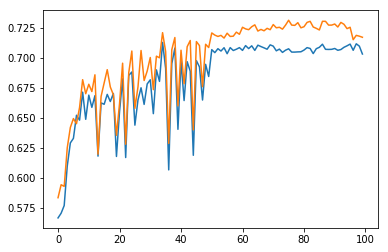
\includegraphics[width=0.8\textwidth]{value_iter_line}
    \bicaption{文本匹配算法的准确率变化曲线}{Accuracy curve of text matching MDP}
    \label{fig:value_iter_line}
\end{figure}

为了测试向前看的单词个数$m$对于算法性能的影响,我们对向前看 2,3,4,5 个单词分别进行了实验。实验结果如下:

\begin{table}[!htbp]
    \bicaption{向前看的单词数量对算法性能影响}{The influence of looking forward words count to our algrithm}
    \label{tab:MDP_forwrd_word}
    \centering
    \footnotesize% fontsize
    \setlength{\tabcolsep}{4pt}% column separation
    \renewcommand{\arraystretch}{1.2}%row space
    \begin{tabular}{cccc}
        \hline
        \multirow{2}{*}{向前看单词个数} &
        \multicolumn{3}{c}{\multirow{1}{*}{Evaluation Criterion}} \\
        \cline{2-4} & acc & F1 & auc \\
        \hline
        $k=2$ & $0.7280$ & $0.7425$ & $0.8072$ \\
        $k=3$ & $\textbf{0.7345}(*)$ & $\textbf{0.7417}(*)$ & $\textbf{0.8149}(*)$ \\
        $k=4$ & $0.7311$ & $0.7338$ & $0.8112$\\
        $k=5$ & $0.7280$ & $0.7366$ & $0.8067$\\
        \hline
    \end{tabular}
\end{table}

可以发现 $m=3$ 时算法的表现最优。这是因为一般情况下来说,语言的组合结构问题构成的词语个数都是有限的,一般都在3,4个左右。在 $m=2$ 时,无法覆盖大部分的次序颠倒的场景;在 $m$大于3时,算法的各项指标都开始逐渐下滑。这可能是因为在 $m$ 过大后,截取到的句子长度远大于次序颠倒部分的长度,使得神经网络捕捉到的信息中更多的包含了序列信息,次序颠倒信息的比重下降。

\begin{figure}[H]
    \centering
    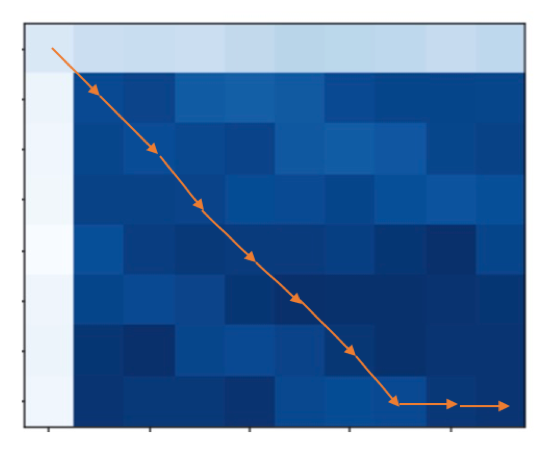
\includegraphics[width=0.5\textwidth]{val_iter_path}
    \bicaption{值迭代生成的路径}{Path generated by value iteration}
    \label{fig:val_iter_path}
\end{figure}

图\ref{fig:val_iter_path} 展示了在输入样本为 $Q$=What are some examples of acidic substances?,$D$=What are some examples of substances soluble in water? 值迭代的生成路径。由于每个方向的值都可以由其左边、上边、和左上的方块得到,因此我们在画图时将3个值取平均作为这个方块的值。从图中我们可以明显发现,右下角为颜色最浓的部分,右上和左下的颜色相对来说都要淡很多。

但是由于值迭代基于贪心的策略导致算法很容易陷入过拟合,为了测试VIM算法的小数据集上的效果,我们在Quora数据集上选取了10240个句子对进行测试。测试方法同样采用五折交叉验证:

\begin{table}[H]
    \bicaption{VIM算法在 Quora 小数据集上的测试结果}{The result of VIM algorithm on small Quora dataset}
    \label{tab:MDP_small_test}
    \centering
    \footnotesize% fontsize
    \setlength{\tabcolsep}{4pt}% column separation
    \renewcommand{\arraystretch}{1.2}%row space
    \begin{tabular}{cccc}
        \hline
        \multirow{2}{*}{Algorithm} &
        \multicolumn{3}{c}{\multirow{1}{*}{Evaluation Criterion}} \\
        \cline{2-4} & acc & F1 & auc \\
        \hline
        VIM with $\epsilon$ = 0 & $0.6465$ & $0.6644$ & $0.7056$ \\
        VIM with $\epsilon$ = 0.1 & $0.6519$ & $\textbf{0.6772}(*)$ & $0.7080$ \\
        VIM with changed $\epsilon$ & $0.6532$ & $0.6612$ & $0.7147$ \\
        \hline
        MatchPyramid & $\textbf{0.6671}(*)$ & $0.6702$ & $0.7237$ \\
        \hline
        MatchSRNN & $0.6617$ & $0.6736$ & $\textbf{0.7285}(*)$\\
        \hline
    \end{tabular}
\end{table}

从表格 \ref{tab:MDP_small_test} 可以发现,在小数据集下 VIM 算法出现了明显的过拟合,人工调节的 $\epsilon$ 可以小幅度提高算法的效果,但是仍然无法超过 MatchPyramid 和 MatchSRNN。

\section{本章小结}
本章主要介绍了文本匹配的马尔科夫决策过程。首先介绍了马尔科夫决策过程的背景,包括马尔科夫链以及马尔科夫决策过程的训练和推断,并且根据文本匹配的场景对文本匹配的MDP进行了形式化描述,并利用值迭代的方法进行训练和推断。该模型在大数据量的情况下表现优异,但是由于值迭代算法的缺陷,在小数据场景下表现不佳。在后续章节中,本文将针对该问题进行改进。

\chapter{基于蒙特卡罗树搜索的模式文本匹配}
\label{chap:Zero}
利用 value iteation 可以解决大部分文本匹配的问题,但是 value iteration 基于贪心的路径搜索难以解决语言的组合结构问题。对于词序的微小变化导致的语义差别, value iteration 往往难以识别。而且 value iteration 在小数据集下容易陷入局部最优而导致算法严重过拟合。而 AlphaGo 以及 AlphaGo Zero 通过引入蒙特卡罗搜索树很好地解决了路径搜索中的贪心导致的局部最优解问题。本章介绍了蒙特卡罗树搜索相关算法并提出了基于蒙特卡罗树搜索的文本匹配算法。

\section{蒙特卡罗树搜索增强的马尔科夫决策过程介绍}
\subsection{蒙特卡罗树搜索介绍}\label{sec:MCTS_intro}
蒙特卡罗树搜索\cite{Coulom2006EfficientSA} 在 2006 年被提出并在过去十多年中广泛用于各种游戏的人工智能\cite{Lorentz2008AmazonsDM, Enzenberger2010FuegoA,Buro2009ImprovingSE}。蒙特卡罗树搜索每次循环包含四步:

1. 选择(selecion):从根节点 R 开始,依次选择最佳的子节点,直到达到叶节点。选择最佳子节点的难点主要在于为了探索解空间需要维持较高的探索次数和利用现有模拟结果以加快训练速度。第一次解决探索和利用平衡的方法被称为上限置信区间算法\cite{Kocsis2006BanditBM}(Upper Confidence Bound 1 applied to trees),该方法基于 UCB1 \cite{Auer2002FinitetimeAO},建议在选择子节点时,以最大化 $\frac{w_i}{n_i} + c\sqrt{\frac{\ln N_i}{n_i}}$ 为目标。式中 $w_i$ 表示第 $i$ 次移动后的取胜次数;$n_i$ 表示第 $i$ 次移动后的仿真次数; $N_i$ 表示总仿真次数, $c$ 表示探索参数。

2. 扩展(expansion): 如果游戏没有结束,那么扩展叶节点,将一个或多个可用节点添加为该叶节点的子节点,并选择其中的一个子节点作为节点 C 。

3. 仿真(simulation): 从节点 C 开始,用随机策略选择节点进行游戏。

4. 反向传播(Backpropagation):根据仿真的结果更新从 C 到 R 的节点。

\begin{figure}[H]
    \centering
    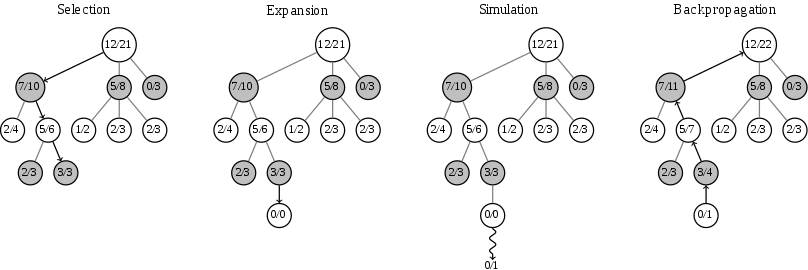
\includegraphics[width=1.0\textwidth]{MCTS}
    \bicaption{蒙特卡洛搜索树步骤}{Each Step of Monte Carlo tree search}
    \label{fig:MCTS}
\end{figure}

\subsection{围棋中的蒙特卡罗树搜索增强}
\label{sec:AlphaGo}
AlphaGo 算法中存在 3 个网络:使用监督学习训练的策略网络 $p_\sigma$ 以及该网络的简化版 $p_\pi$;使用强化学习训练的策略网络 $p_\rho$ 以及价值网络 $v_\theta$。在树搜索的过程中,$p_\sigma$ 被用作模拟人类棋手落子;$p_\rho$ 决定落子位置,$v_\theta$ 判断当前局势。

$p_\sigma$ 的训练数据来自于 KGS 的三千万棋局,利用每个棋局及其对应的落子的数据,训练得到概率分布 $p_\sigma(a|s)$,即在当前状态(棋局)下采取行动(落子)的概率。由于 $p_\sigma$ 网络结构比较复杂,推导速度较慢,因此在 AlphaGo 算法训练时采用简化网络 $p_\pi$ 以降低训练速度;推导时采用 $p_\sigma$以提高胜率。

\begin{figure}[!htbp]
    \centering
    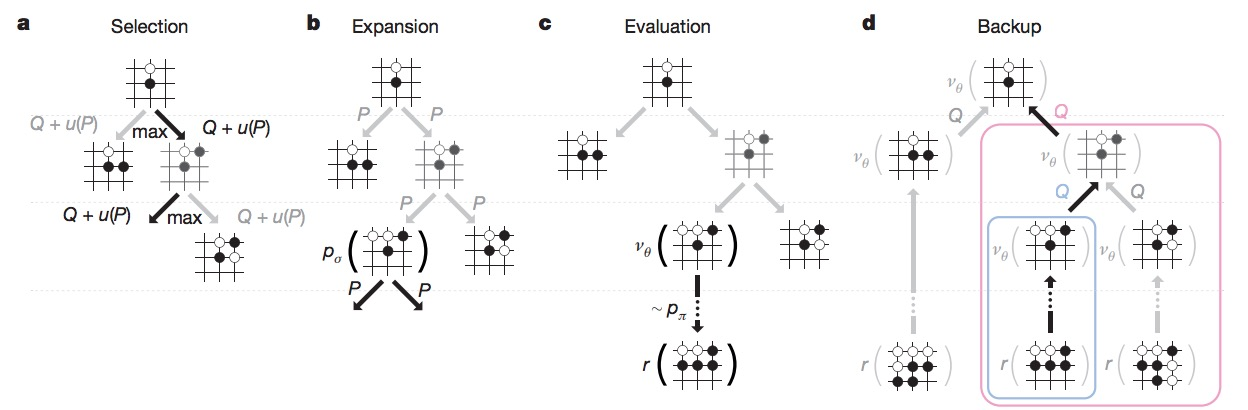
\includegraphics[width=1.0\textwidth]{Alpha_Go}
    \bicaption{AlphaGo 的树搜索过程}{Monte Carlo tree search in AlphaGo}
    \label{fig:Alpha_Go}
\end{figure}

蒙特卡罗树搜索使用随机进行仿真,Alpha Go 利用价值网络辅助策略网络作为落子参考进行仿真。图 \ref{fig:Alpha_Go} 中每一条边$(s, a)$ 都包含了行动价值$Q(s,a)$,该节点的访问次数$N(s,a)$以及先验概率$P(s,a) = p_\sigma(a|s)$。每次仿真从根节点开始根据当前状态 $s_t$ 选择行动 $a_t$ 直至到达叶节点。

\begin{equation}
\begin{aligned}
&a_t = \arg\max_a(Q(s_t,a) + u(s_t,a)) \\
&u(s_t,a) \propto \frac{P(s,a)}{1+N(s,a)}
\end{aligned}
\end{equation}

叶节点的重要程度由价值网络$v_\theta$ 和策略网络 $p_\pi$ 输出 $z_L$ 确定。

$$
V(s_L) = (1-\lambda)v_\theta(s_L) + \lambda z_L
$$

模拟结束时,所有边的行动价值以及参观次数都会被更新。
$$
\begin{aligned}
N(s,a) &= \sum_{i=1}^N\mathbf{1}(s,a,i)
Q(s,a) &= \frac{1}{N(s,a)}\sum_{i=1}^N\mathbf{1}(s,a,i)V(s_L^i)
\end{aligned}
$$

式中 $s_L^i$ 表示第 $i$ 次仿真的叶节点, $\mathbf{1}(s,a,i)$ 表示边 $(s,a)$ 是否被访问过。

AlphaGo Zero 是对 AlphaGo 的改进。相对于 AlphaGo,AlphaGo Zero 主要改进了以下几点:

1. AlphaGo Zero 是一个自训练的强化学习过程,不需要任何人类的先验知识;

2. AlphaGo Zero 仅仅使用围棋棋盘的黑白子作为输入,不需要其他人工抽取的特征;

3. AlphaGo Zero 将策略和价值网络融合,增强了网络的泛化能力;同时使用深度残差网络,网络深度加深,扩展了网络的解释能力;

AlphaGo Zero 使用了一个参数为 $\theta$ 的深度网络 $f_\theta$ ,该网络将棋盘作为输入,输出对应的概率和值函数 $(\mathbf{p}, v) = f_\theta(s)$. 式中 $\mathbf{p}$ 表示行动(落子)的概率$p_a = Pr(a|s)$, $v$ 是一个标量,表示当前棋局的胜率。

深度网络的训练仍然采用蒙特卡罗树搜索的方式。在时刻 $t$, 使用 $f_\theta$ 的输出为作参考进行下一轮蒙特卡罗树搜索,每一轮的树搜索都会输出当前状态(棋局)下每个行动(落子)的概率 $\mathbf{\pi}$。蒙特卡罗树搜索得到的落子概率比直接$f_\theta$  得到的落子概率更强,因此蒙特卡罗树搜索可以被认为是一个策略提升(policy improvement)的过程。利用$\mathbf{\pi}$进行落子后,不断循环直到棋局结束。在棋局结束后,将对弈者的胜负情况 $z$ 作为价值更新参数。最后更新$f_\theta$的网络参数以让 $f_\theta$ 的输出的落子概率和胜率 $(\mathbf{p}, v)$ 尽可能接近 $(\mathbf{\pi}, z)$,并在后面的棋局中使用新的参数来进行自对弈。

$f_\theta$ 的损失函数为:
$$
\ell = (z-v)^2 + \mathbf{\pi}^T\log \mathbf{p} + c\|\theta\|^2
$$
其中 $c$ 是正则化的系数。

蒙特卡罗树搜索以及参数更新的相关部分参考 \ref{sec:AlphaGo} 节。

\section{基于蒙特卡罗树搜索的文本匹配算法介绍}
在上一章,本文对文本匹配算法的 MDP 进行了介绍。受到 AlphaGo 和 AlphaGo Zero 的启发,本章尝试将蒙特卡罗树搜索方法应用于文本匹配中。我们将本章提出的方法称为 MM-Match。

\begin{figure}[!htbp]
    \centering
    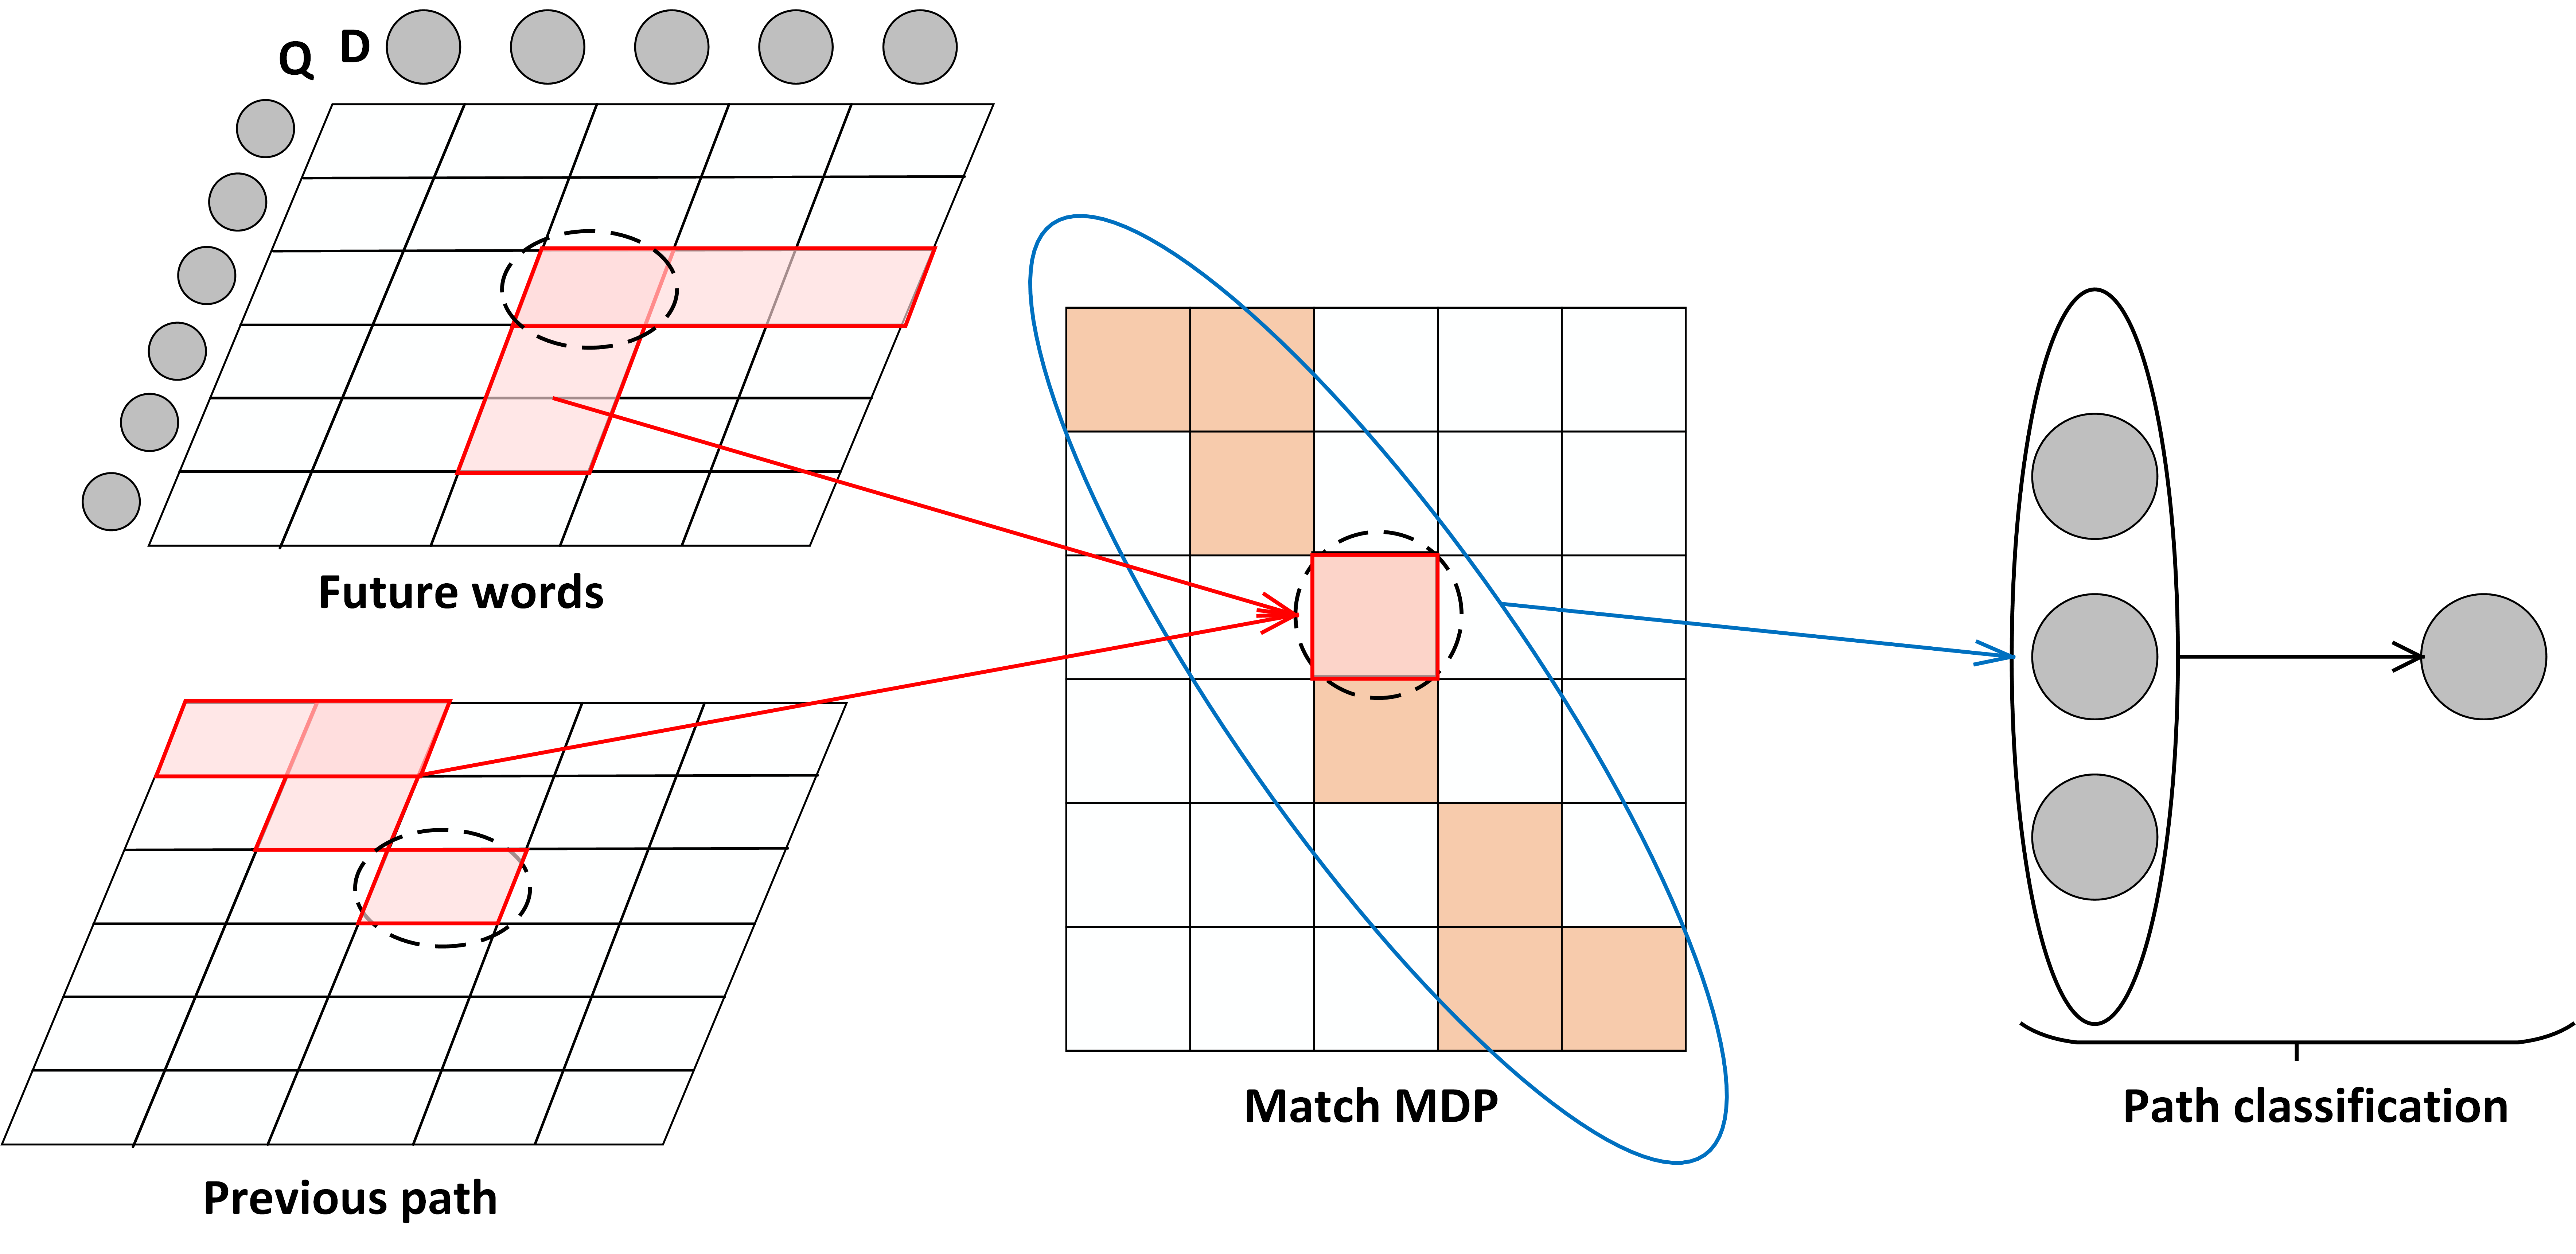
\includegraphics[width=0.8\textwidth]{grid}
    \bicaption{MM-Match 算法结构}{The architecture of MM-Match}
    \label{fig:MCTS_sum}
\end{figure}

\subsection{文本匹配 MDP 改进}
本节主要介绍对 \ref{sec:TM_MDP} 节所提到的 MDP 过程的改进。算法的整体流程和 \ref{sec:TM_MDP} 节相比没有太大改进,仍然是先生成匹配路径之后基于生成的路径判断是否匹配。

1. 状态 $\mathcal{S}$:我们将在 $t$ 时刻的状态 $s_t$ 定义为当前的路径以及从当前位置开始向前看的 $k$ 个单词:
$$
\begin{aligned}
\mathbf{Q}_t &= \{\mathbf{u}_{q_1}, \mathbf{u}_{q_2}, \mathbf{u}_{q_3}, \cdots, \mathbf{u}_{q_t}\},\\
\mathbf{D}_t &= \{\mathbf{v}_{d_1}, \mathbf{v}_{d_2}, \mathbf{v}_{d_3},\cdots, \mathbf{v}_{d_t}\},\\
\mathbf{F}_t &= \{[\mathbf{u}_{q_t}, \mathbf{v}_{d_t}], [\mathbf{u}_{1+q_t},\mathbf{v}_{1+d_t}] \cdots, [\mathbf{u}_{k+q_t}, \mathbf{v}_{k+d_t}]\},\\
s_t &= [\mathbf{Q}_t, \mathbf{D}_t, \mathbf{F}_t]
\end{aligned}
$$
式中 $q_t$ 和 $d_t$ 仍然表示当前位置, $\mathbf{Q}_t$ 和 $\mathbf{D}_t$ 表示输入的句子对 $Q, D$ 的前 $q_t$ 和 $d_t$ 按照路径拉伸得到的序列,$\mathbf{F}_t$ 表示从当前位置 $q_t, d_t$ 向前看 $k$ 个单词得到的序列。

2. 动作$\mathcal{A}$:在每个时间 $t$,我们都可以选择向下,向右或者像右下方行走。

3. 状态转移函数$\mathcal{T}(S,\mathcal{A})$:状态转移函数 $\mathcal{T}:S\times \mathcal{A}\rightarrow S$ 被定义为:
$$
(q_{t+1}, d_{t+1}) =
\begin{cases}
(q_{t} + 1, d_{t}) &\text{if goes down} \\
(q_{t}, d_{t} + 1) &\text{if goes right}  \\
(q_{t} + 1, d_{t} + 1) &\text{if goes obliquely}
\end{cases} \\
$$
$$
\begin{aligned}
s_{t+1} &= \mathcal{T}(s_t, a_t) = \mathcal{T}([\mathbf{Q}_t, \mathbf{D}_t, \mathbf{F}_t], a_t) = [\mathbf{Q}_{t+1}, \mathbf{D}_{t+1},\mathbf{F}_{t+1}]
\end{aligned}
$$
在每个时间 $t$:系统根据当前的状态选择一个行动(移动方向),并根据方向移动到下一个位置,状态随之转移:将当前位置两个句子的词向量分别添加到对应路径的末尾,更新未来单词序列。完成转移后,再根据当前状态继续移动。

4.值函数 $V$:值函数 $V: S\rightarrow \mathbb{R}$ 是对当前模型是否可以得到正确预测结果的预测。值函数需要不断更新以更加准确的得到预测结果。本节提出的值函数需要用到2个LSTM将 $Q_t$ 和 $D_t$ 映射为2个一维向量,并将结果定义为对这两个向量加权和的非线性转换:
\begin{equation}
\label{eq:MCTS_value}
V(s) = \sigma (<\mathbf{w}, \mathbf{g}_v(s)> + \mathbf{b}_v)
\end{equation}

式中 $\mathbf{w}, \mathbf{b}_v$ 是需要学习的参数,$
\sigma(x) = \frac{1}{1+e^{-x}}$ 是 sigmoid 函数以输出一个 0 $\sim$ 1 之间的概率,$\mathbf{g}_v(s)$ 是对将 LSTM$_Q$ 以及 LSTM$_D$ 的最后一层隐向量连接得到的:

\begin{equation}
\mathbf{g}_v(s) = [\mathrm{LSTM}_Q(\mathbf{Q}_t)^T, \mathrm{LSTM}_D(\mathbf{D}_{t})^T]^T
\end{equation}

LSTM 网络的定义和公式~\ref{eq:LSTM} 一致,LSTM$_Q$ 和 LSTM$_D$ 共享参数。

5. 策略函数 $\mathbf{\pi}$:$\mathbf{\pi}(s)$ 将环境状态作为输入,输出每个行动的概率。策略函数将 $\mathbf{g}_v(s), F_t$ 作为输入,使用一个 LSTM 将 $F_t$ 映射为一个一维向量,并将其和 $\mathbf{g}_v(s)$ 连接,将连接后的向量利用 softmax 函数进行归一化得到每个行动的概率分布:
\begin{equation}
\label{eq:MCTS_policy}
\begin{aligned}
\pi(a|s) &= \frac{\exp\left\{\Phi(a)^T \mathbf{U}_\pi ~\mathbf{g}_\pi(s)\right\}}{\sum_{a'\in\mathcal{A}(s)} \exp\left\{\Phi(a')^T \mathbf{U}_\pi ~\mathbf{g}_\pi(s)\right\}} \\
\mathbf{g}_\pi(s) &= [\mathbf{g}_v(s) , \mathrm{LSTM}_F(\mathbf{F}_{t})^T]^T
\end{aligned}
\end{equation}

\subsection{路径判别}
在 \ref{sec:path_classify} 中,我们提出了一种针对于路径的判别模型判断路径是否匹配。但是由于该方法在每次运行时的计算图都不尽相同,因此效率很低。本节对该方法进行了改进以提高其训练和推断速度。

判别模型将 $\mathbf{Q}_t$ 和 $\mathbf{D}_t$ 作为输入,并使用两个 LSTM 将其映射为2个矩阵,最后使用一个 LSTM 接受两个矩阵作为输入,输出一个一维向量:
$$
\begin{aligned}
\mathbf{g}_q &= \mathrm{LSTM}_Q(Q_t)\\
\mathbf{g}_d &= \mathrm{LSTM}_D(D_t)\\
\mathbf{g}_c^{\text{in}} &= [[\mathbf{g}_{q, 1}, \mathbf{g}_{d, 1}], [\mathbf{g}_{q, 2}, \mathbf{g}_{d, 2}], \cdots, [\mathbf{g}_{q, t}, \mathbf{g}_{d, t}]]\\
\mathbf{g}_c^{\text{out}} &= \mathrm{LSTM}_C({g}_c^{\text{in}})
\end{aligned}
$$
LSTM$_Q$和LSTM$_D$ 共享参数。最后输出概率会通过 sigmoid 函数变换概率输出:
\begin{equation}
\label{eq:classification_model}
p_m = \frac{1}{1+e^{-{\mathbf{g}_c^{\text{out}}}}}
\end{equation}

\begin{figure}[!htbp]
    \centering
    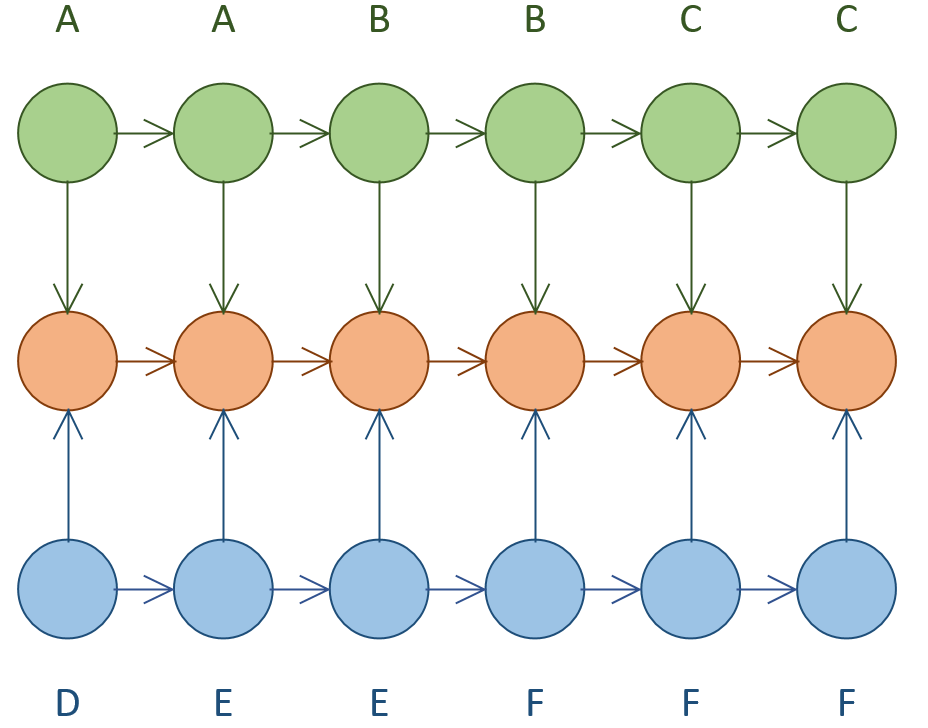
\includegraphics[width=0.4\textwidth]{MCTS_path}
    \bicaption{路径判别函数}{Path classifiction}
    \label{fig:MCTS_path}
\end{figure}

\subsection{蒙特卡罗树搜索的训练和推断}
\label{sec:MCTS_train}
在\ref{sec:lab_value} 节,本文通过在大数据和小数据集上的训练结果发现单纯将策略函数的输出作为行动概率很容易陷入局部最优解,即使使用 $\epsilon$-贪心的方式也很难摆脱。受 AlphaGo 和 AlphaGo Zero 的启发,本节使用蒙特卡罗树搜索的方式进行前向式搜索。在 $t$ 时刻,算法在策略和价值网络的辅助下执行一次蒙特卡罗树搜索,得到搜索策略 $\mathbb{\pi}$,并根据 $\pi$ 确定下一个行动的位置。

\begin{algorithm}[!htbp]
\caption{TreeSearch}\label{alg:TreeSearch}
\renewcommand{\algorithmicrequire}{\textbf{Input:}}
\renewcommand{\algorithmicensure}{\textbf{Output:}}
\begin{algorithmic}[1]
\Require root $s_R$, value $V$, policy $\pi$, search times $K$
\Ensure Search policy $\mathbf{\pi}$
\For{$k = 0$~$\text{to}$~$K-1$}
\State $s_L\leftarrow s_R$
\State {\{Selection\}}
\While{$s_L \textrm{ is not a leaf node}$}
  \State $a \leftarrow \arg\max_{a\in\mathcal{A}(s_L)} Q(s_L, a) +\lambda \cdot U(s_L, a)$\Comment{Eq.~(\ref{eq:Selection})}
  \State $s_L \leftarrow \textrm{ child node pointed by edge }(s_L, a)$
\EndWhile

\State {\{Evaluation and expansion\}}
%\IF{$s_L$ can be expanded}
    \State $v\leftarrow V(s_L)$ \Comment{simulate $v$ with value function $V$}
  \For{$\text{all }a \in\mathcal{A}(s_L)$}
    \State Expand an edge $e$ to node $ s = [s_L.\mathbf{Q}_t, s_L.\mathbf{D}_t, s_L.\mathbf{F}_t]$
    \State $e.P \leftarrow p(a|s_L); e.Q \leftarrow 0; e.N \leftarrow  0$\Comment{init edge properties}
  \EndFor
%\ELSE
% \State{$v\leftarrow\left\{\begin{array}{cl} V(s_L) & R= NULL\textrm{ or }J=\emptyset \\ R(s_L.\mathcal{Z}, J) & \textrm{others}\\ \end{array} \right.$}\Comment{simulate with $V$ at test phase ($R=NULL$ or $J=\emptyset$), or directly set to its real value (e.g., $\alpha$-NDCG) at the training phase}
%\ENDIF
\State {\{Back-propagation\}}
\While{$s_L \neq s_R$}
  \State $s \leftarrow \textrm{ parent of }s_L; e \leftarrow \textrm{ edge from }s\textrm{ to }s_L$
  \State $e.Q \leftarrow \frac{e.Q\times e.N + v}{e.N + 1}$\Comment{Equation~(\ref{eq:UpdateQN})}
  \State $e.N \leftarrow e.N + 1; s_L \leftarrow s$
\EndWhile
\EndFor

\State {\{Calculate tree search policy. Eq.~(\ref{eq:SearchProb})\}}
\For{$\text{all }a\in\mathcal{A}(s_R)$}
  \State $\pi(a|s_R)\leftarrow \frac{e(s_R, a).N}{\sum_{a'\in\mathcal{A}(s_R)}e(s_R, a').N}$
\EndFor
\Return $\mathbf{\pi}$
\end{algorithmic}
\end{algorithm}

Alg~\ref{alg:TreeSearch} 展示了蒙特卡罗树搜索的细节,其中每一个树节点对应一个状态。算法以根节点 $s_R$、值函数 $\mathcal{V}$ 以及策略函数 $\pi$ 作为输入,输出策略 $\mathbb{\pi}$。算法会迭代 $K$ 次,每次从 $s_P$ 开始选择一个方向移动。搜索树中每条边$e(s,a)$都存储着行动价值 $Q(s,a)$ 参观次数 $N(s,a)$ 以及先验概率 $\pi(s,a)$。每次迭代式,会执行以下操作:

1. 选择:每次迭代都从根节点 $s_R$ 开始,以最大化上限置信区间为目标选择行动:
\begin{equation}\label{eq:Selection}
  a_t = \arg\max_a (Q(s_t, a) + \lambda U(s_t, a)),
\end{equation}
式中 $\lambda >0$ 是权衡系数,$U(s_t, a) =  p(a|s_t)\frac{\sqrt[]{\sum_{a'\in\mathcal{A}(s_t)} N(s_t, a')}}{1 + N(s_t, a)}$. $U(s_t, a)$ 和先验概率有关但是随着参观次数的增加而逐渐减小。

2. 评价扩展:到达叶节点时,节点会根据值函数 $V(s_L)$ (公式~\ref{eq:MCTS_value}) 计算当前节点的价值。如果搜索过程没有结束,则该节点需要被扩展。新的叶节点状态 $s_L$ 会被初始化为 $\pi(s_L, a) =\pi(a|s_L)$ (公式~\ref{eq:MCTS_policy}), $Q(s_L, a)= 0$, $N(s_L, a) = 0$。本节介绍的算法会始终扩展叶节点直到到达矩阵右下角。

3. 回溯更新:评价结束时,每条边都会被更新:
\begin{equation}
\label{eq:UpdateQN}
\begin{aligned}
  &Q(s, a) \leftarrow  \frac{Q(s, a) \times N(s, a) + V(s_L)}{N(s, a) + 1}\\
  &N(s, a) \leftarrow  N(s, a) + 1.
\end{aligned}
\end{equation}

4. 计算策略:在 $K$ 次迭代结束后,根据根节点 $s_L$ 每条边的访问次数确定每个行动的概率:
\begin{equation}\label{eq:SearchProb}
\pi(a|s_R) = \frac{N(s_R, a)^{\frac{1}{\tau}}}{\sum_{a'\in\mathcal{A}(s_R)} N(s_R, a')^{\frac{1}{\tau}}},
\end{equation}
式中 $\tau > 0$ 表示系统温度。

\subsubsection{模型的训练}
本章提出的模型的参数 $\Theta_{MCTS}$(包含 $\mathbf{w}, b_v, \mathbf{U}_p$, 以及 LSTM$_D$, LSTM$_Q$ 和 LSTM$_F$中的参数),$\Theta_{c}$(包含LSTM$_D$, LSTM$_Q$ 和 LSTM$_c$ 中的参数)需要在训练时被更新。在训练阶段,算法接受 $N$ 个标记的句子对 $D = \{ (\mathbf{Q}^{(n)}, \mathbf{D}^{(n)}), \mathbf{Y}\}_{n=1}^{N}$。算法~\ref{alg:Train}展示了整个训练过程。首先将参数  $\Theta_{MCTS}$ 和 $\Theta_{c}$ 初始化为 $[-1, 1]$ 的随机数,每轮迭代时,对于每个句子对 $(\mathbf{Q}, \mathbf{D})$,我们都需要预测一条路径。在每个时间 $t$都会执行一次蒙特卡洛树搜索,并输出策略 $\mathbb{\pi}$,根据策略随机采样出对应的移动方向 $a_t$,直到到达匹配矩阵的右下角。在得到一条路径 $([u_{q_1}, u_{q_2}, \cdots, u_{q_t}], [v_{d_1}, v_{d_2}, \cdots, v_{d_t}])$ 后,使用交叉熵损失更新路径判别模型:

\begin{equation}
\label{eq:classification_loss}
\ell_c(Y, p) = -\left(Y\log(p) + (1-Y)\log (1-p)\right)
\end{equation}

在路径判别模型收敛后,对每条路径进行预测得到标签 $Y_p$,并根据 $Y_p$ 与实际标签 $Y$ 计算奖励 $r= \mathbb{I}_{\mathbf{Y} = \mathbf{Y}_p}$。蒙特卡罗树搜索中每一轮生成的数据 $E=\{s_t, \mathbb{\pi}_t\}$ 以及 $r$ 会被用作更新价值和策略网络,使其输出的值 $V(s_t)$和策略$\mathbb{p}(s_t)$ 尽可能逼近 $r$ 和 $\mathbb{p}(s_t)$。该网络的损失函数为:
\begin{equation}
\label{eq:loss}
\begin{aligned}
  \ell(E, r) = &\sum_{t=1}^{|E|} (-(r\log V(s_t) + (1-r)\log (1-V(s_t)))  \\
  &+ \beta\sum_{a\in\mathcal{A}(s_t)}\pi_t(a|s_t) \log \frac{1}{\pi(a|s_t)}).
\end{aligned}
\end{equation}
模型通过反向传播和离散梯度下降更新。

\begin{algorithm}[!htbp]
\caption{Train MM-Match}\label{alg:Train}
\renewcommand{\algorithmicrequire}{\textbf{Input:}}
\renewcommand{\algorithmicensure}{\textbf{Output:}}
\begin{algorithmic}[1]
\Require Labeled data $D=\{ (\mathbf{D}^{(n)}, \mathbf{Q}^{(n)}, \mathbf{Y}^{(n)})\}_{n=1}^N$, learning rate $\eta$, number of search $K$
\Ensure $\Theta_{MCTS}, \Theta_{c}$
\State \text{Initialize} $\Theta_{MCTS}, \Theta_{c} \leftarrow$ random values in $[-1, 1]$
\Repeat
  \For{$(\text{all }\mathbf{X}, \mathbf{Y})\in D$}
    \State {$s \leftarrow [\{\mathbf{u}_1\}, \{\mathbf{v}_1\}, \{[\mathbf{u}_1,\mathbf{v}_1], \cdots, [\mathbf{u}_k, \mathbf{v}_k]\}]$}
    \While{not reach right down corner}
            \State $\mathbb{\pi} \leftarrow \mathrm{TreeSearch}(s, V, \mathbf{p}, K)$ \Comment{Alg.~(\ref{alg:TreeSearch})}
      \State sample action ${a\in\mathcal{A}(s)}$ according to $\pi(a|s)$
      \State $E\leftarrow E \oplus \{(s, \mathbb{\pi})\}$
      %\State $[\mathbf{q}, \mathcal{Z}, X]\leftarrow s$
      \State $s \leftarrow [s.\mathbf{Q}_{t+1}, s.\mathbf{D}_{t+1}, s.\mathbf{F}_{t+1}]$
    \EndWhile
    \While{\text{not convergence}}
    \State $\Theta_{c} \leftarrow \Theta_{c} - \eta \frac{\partial \ell_c(\mathbf{Y}, p)}{\partial \Theta_{c}}$  \Comment{$\ell_c$ is defined in Eq.~(\ref{eq:classification_loss})}
    \EndWhile
    \State compute $\mathbf{Y}_p$ by Eq.~(\ref{eq:classification_model})
    \State $r \leftarrow \mathbb{I}_{\mathbf{Y} = \mathbf{Y}_p}$
    \State $\Theta_{MCTS} \leftarrow \Theta_{MCTS} -\eta \frac{\partial \ell(E, r)}{\partial \Theta_{MCTS}}$ \Comment{$\ell$ is defined in Eq.~(\ref{eq:loss})}
  \EndFor
\Until {converge}
\State\Return $\Theta_{MCTS}, \Theta_{c}$
\end{algorithmic}
\end{algorithm}

\subsubsection{模型的推断}
算法~\ref{alg:Train}展示了模型的推断过程。给定一个句子对 $\mathbf{Q}, \mathbf{D}$,系统的初始化状态 $s_1=[\{\mathbf{u}_1\}, \{\mathbf{v}_1\}, \{[\mathbf{u}_1,\mathbf{v}_1], \cdots, [\mathbf{u}_k, \mathbf{v}_k]$。在每个时间节点 $t$,主体都会得到系统的状态 $s_t=[\mathbf{Q}_t, \mathbf{D}_t, \mathbf{F}_t]$ 以及蒙特卡罗树搜索得到的策略 $\mathbb{\pi}$,根据 $\mathbb{\pi}$ 做出行动后更新当前状态得到 $s_{t+1}$。该过程不断持续直到到达匹配矩阵的右下角。

\begin{algorithm}[!htbp]
\caption{Text MM-Match}\label{alg:RLRank_MCTS}
\renewcommand{\algorithmicrequire}{\textbf{Input:}}
\renewcommand{\algorithmicensure}{\textbf{Output:}}
\begin{algorithmic}[1]
\Require sentence pair $\mathbf{Q}=\{\mathbf{u}_1, \cdots, \mathbf{u}_M\}$, $\mathbf{D}=\{\mathbf{w}_1, \cdots, \mathbf{w}_M\}$, value function $V$, policy function $\mathbf{p}$, and search times $K$,
\Ensure label $\mathbf{Y}$
\State $s \leftarrow [\{\mathbf{u}_1\}, \{\mathbf{v}_1\}, \{[\mathbf{u}_1,\mathbf{v}_1], \cdots, [\mathbf{u}_k, \mathbf{v}_k]\}]$
\While{not reach right down corner}
  \State $\mathbb{\pi} \leftarrow \mathrm{TreeSearch}(s, V, \mathbf{p}, K)$
  \State $a \leftarrow \arg\max_{a\in\mathcal{A}(s)} \pi(a|s)$
% \State $[\mathbf{X}, \mathbf{Y}]\leftarrow s$
  \State $s \leftarrow [s.\mathbf{Q}_{t+1}, s.\mathbf{D}_{t+1}, s.\mathbf{F}_{t+1}]$
\EndWhile
\State compute $\mathbf{Y}_p$ by Eq.~(\ref{eq:classification_model})
\State \Return $\mathbf{Y_p}$
\end{algorithmic}
\end{algorithm}


\section{实验分析}
为了对我们提出的基于蒙特卡罗树搜索的文本匹配算法有效性进行评估,我们利用 Quora 的问题匹配数据集进行了测试。实验设置和 \ref{sec:lab_value} 节相同。由于蒙特卡洛树搜索的时间较长,因此我们只在小数据集上进行的测试。

\begin{table}[H]
    \bicaption{基于蒙特卡罗树搜索的文本匹配算法测试结果}{The result of text matching algorithm based on MCTS on Quora dataset}
    \label{tab:MCTS_small_test}
    \centering
    \footnotesize% fontsize
    \setlength{\tabcolsep}{4pt}% column separation
    \renewcommand{\arraystretch}{1.2}%row space
    \begin{tabular}{cccc}
        \hline
        \multirow{2}{*}{Algorithm} &
        \multicolumn{3}{c}{\multirow{1}{*}{Evaluation Criterion}} \\
        \cline{2-4} & acc & F1 & auc \\
        \hline
        MM-Match & $\textbf{0.6776}(*)$ & $\textbf{0.6845}(*)$ & $\textbf{0.7371}(*)$ \\
        \hline
        MatchPyramid & $0.6671$ & $0.6702$ & $0.7237$ \\
        \hline
        MatchSRNN & $0.6617$ & $0.6736$ & $0.7285$\\
        \hline
    \end{tabular}
\end{table}

可以发现MM-Match在3个评价指标上均大幅度领先于 MatchPyramid 和 MatchSRNN。

从收敛速度上来看,我们的算法继承了算法\ref{alg:TM_train} 的优点,收敛速度同样很快。类似的,我们也在上面实验中的一折数据上统计了验证集和测试集的auc随轮数的变化情况:

\begin{figure}[H]
    \centering
    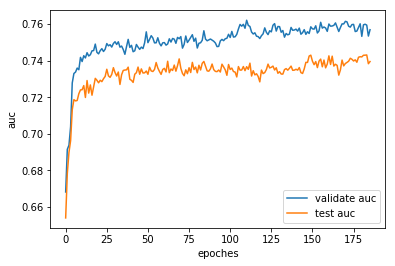
\includegraphics[width=0.8\textwidth]{MCTS_line}
    \bicaption{MM-Match算法auc变化曲线}{Auc curve of MM-Match}
    \label{fig:MCTS_line}
\end{figure}

观察图\ref{fig:MCTS_line} 可以发现,MM-Match 的收敛速度明显快于 VIM,算法在20轮不到就已经收敛。

为了实际查看蒙特卡罗树搜索访问的节点,我们将算法 \ref{alg:TreeSearch} 访问节点数可视化:

\begin{figure}[H]
    \centering
    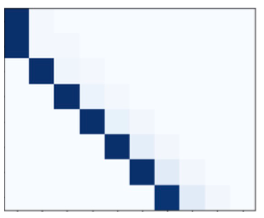
\includegraphics[width=0.4\textwidth]{MCTS_exp_path}
    \bicaption{MM-Match树搜索节点访问次数}{Each node visit number in tree search of MM-Match}
    \label{fig:MCTS_exp_path}
\end{figure}

图 \ref{fig:MCTS_exp_path} 是在输入的句子对为 How do I think positive in life? What is the best way to a positive life 的情况下第一次树搜索后各个节点的访问次数,可以发现右上角和左下角明显为空,而对角线处的访问次数明显最高。

\section{本章小结}
本章主要介绍了基于蒙特卡罗树搜索的文本匹配算法。首先我们对上一章提出的 MDP 进行了改进,加入了路径信息。路径信息的引入使得价值网络的预测更加精确。

为了解决直接使用价值网络输出的值函数会导致算法陷入局部最优解的问题,本章引入了蒙特卡罗树搜索算法,通过蒙特卡罗树搜索算法增强搜索策略的可用性,也解决了文本匹配中由于语言组合结构带来的语义区分问题。

最后本文在quora数据集上进行了测试,实验结果表明本文提出的模型具有优异的性能。

\chapter{文本匹配算法的并行实现}

\chapter{总结与展望}
\section{本文总结}
近年来,计算机以及智能终端设备的存储和计算能力不断增强,互联网的信息量呈现爆炸式增长。信息量的增加既为人们的生活带来了便捷,也给人们提出了巨大的挑战。据统计,google每天新增的索引网页页数高达40亿。在海量的信息面前如何高效的获取信息以及如何去除冗余信息成了很多人需要面对的问题。

文本是人类数千年历史中主要的信息载体。虽然移动互联网时代的到来大大方便了视频和音频的传播,但是文本依然是人类目前最普遍和高效的信息获取手段。文本匹配作为信息检索和冗余文本消除的基础技术手段,一直受到学术界和工业界的高度重视。

根据使用场景的不同,文本匹配可以被分为三类:短文本-短文本匹配,短文本-长文本匹配以及长文本-长文本匹配。短文本-短文本的匹配主要用于问答系统、问题复述等领域,先得到句子的矩阵表示后,利用深度网络提取句子的语义信息以及句子间的交互信息,将提取出的信息映射为一个概率分布;短文本-长文本的匹配往往需要用到主题模型等辅助,根据长文本的主题分布判断生成短文本的概率;长文本-长文本的匹配相对较少,同样需要利用主题模型等手段将长文本映射到一个高维向量空间,通过高维向量空间的距离衡量两个文本的相似度。

一个优秀的文本匹配算法一般需要解决三个问题:1) 语言的多义性问题,即相同词语在不同环境下的语义问题;2) 语言的组合结构问题,即相同词语的顺序不同导致的语义不同;3) 匹配的非对称性问题,文本匹配任务中两个句子并不需要语义或者结构一致,如问答系统。

为了解决这些问题,近年来有学者试图将深度学习应用于文本匹配任务,取得了巨大的成功。但是这些方法都试图利用深度学习抽取文本中的语义信息,目前对于计算机来说这仍然是不可能的任务,因此基于深度学习的方法具有天然的局限性。

为了解决上述问题,文本利用强化学习抽取匹配过程中句子之间的交互信息。本文从三个角度出发,解决了利用强化学习抽取交互信息的主要难题。首先,本文针对于文本匹配的场景,利用马尔科夫决策过程建模匹配过程中路径的生成过程,利用值迭代方法对马尔科夫决策过程进行训练和预测,验证了马尔科夫决策过程的正确性;其次,利用蒙特卡罗树搜索向前看的特性解决文本匹配的组合结构问题,取得了良好的效果;最后本文对前面设计算法进行了并行实现,提升了算法的运行速度,为大规模分布式训练奠定了基础。
\section{下一步工作}
本文的工作主要集中于利用强化学习解决文本匹配问题。虽然本文提出的算法可以有效地对文本匹配问题做出判别,但是在实验过程中我们依然发现了一些潜在的问题以及其他的相关研究内容。

1. 强化学习的马尔科夫决策过程改进。
本文利用马尔科夫决策过程抽取了文本匹配过程中的两个句子之间的交互信息,但是这只是对文本匹配过程的一种建模方式。后续研究可以对本文提出的马尔科夫过程进行深入的分析以及进一步的改进。

2. 蒙特卡罗树搜索的并行化探索。
为了提高算法的运行速度,本文针对于文本匹配和蒙特卡罗树搜索的场景设计了并行化搜索的算法。该方法虽然可以有效地提高算法的运行速度,但是在和 Tensorflow 交互的处理上仍然有缺陷。因此可以针对本算法的特殊场景,对 Tensorflow 源代码进行修改,以进一步提升算法的运行速度;同时如何做到实时性仍然是蒙特卡罗树搜索的难点所在。

%---------------------------------------------------------------------------%
% main content
%-
%-> Appendix
%-
%\cleardoublepage%
%\appendix% initialize the environment
%\input{Tex/Appendix}% appendix content
%-
%-> Backmatter: bibliography, glossary, index
%-
\backmatter% initialize the environment
\intotoc{\bibname}% add link to contents table and bookmark
\bibliography{Biblio/ref}% bibliography
% \chapter[附录]{附录\quad 中国科学院大学学位论文撰写要求}\chaptermark{附\quad 录}% syntax: \chapter[toc]{title}\chaptermark{header}

% 学位论文是研究生科研工作成果的集中体现,是评判学位申请者学术水平、授予其学位的主要依据,是科研领域重要的文献资料。根据《科学技术报告、学位论文和学术论文的编写格式》(GB/T 7713-1987)、《学位论文编写规则》(GB/T 7713.1-2006)和《文后参考文献著录规则》(GB7714—87)等国家有关标准,结合中国科学院大学(以下简称“国科大”)的实际情况,特制订本规定。

% \textbf{论文无附录者无需此部分}。

\chapter[致谢]{致\quad 谢}\chaptermark{致\quad 谢}% syntax: \chapter[toc]{title}\chaptermark{header}
\thispagestyle{noheaderstyle}% 如果需要移除当前页的页眉
%\pagestyle{noheaderstyle}% 如果需要移除整章的页眉

转眼间又是一个三年,计算所的学习时光是一段特殊的回忆。在这期间我度过了迷 茫彷徨,也经历了斗志昂扬。但是过往即逝,等待我的是新的征程和新的生活。值此论 文即将完成之际,我要向所有关心和支持我的人们致以最真诚的谢意!

特别感谢我的指导老师徐君老师,您治学严谨,循循善诱,精益求 精的品质与精神,令我倍感钦佩,见贤思齐。研究生期间在您指导和帮助下,我 度过了许多学习和科研的难关;您让我有机会参与开发学科前沿项目,让我体会到了 产学结合的魅力,更是让我在为人处世、团队合作和自我修养等方面都有机会提升。您 的言传身教使我终身受益,我将永远铭记在心。

感谢实验室的师兄师姐们:曾玮、崔国歆、庞亮。在我面 临困难的时候,你们总是耐心地帮我解决一个个难题。不仅佩服你们渊博的学识,更折 服于诸位师兄师姐开放包容的风度。

感谢计算所的各位老师和员工,有高屋建瓴的程学旗老师,诲人不倦的刘悦老 师,和蔼可亲的宋铟老师,风趣幽默的崔连军老师,您们无微不至的帮助与支持,让我 们能够顺利地开展项目开发与研究,不断取得新成果。您们就像勤劳的蜜蜂,兢兢业业, 无私奉献,用辛勤的工作陪伴着我们成长。

感谢在研究生三年中相识的所有同学,特别是陈欣洁、李朝辉、于思皓、冯悦、吴晨、王素、吴志达、陶舒畅、丁汉星、曹家硕、黄冬。每个人身上都有着与众不同的闪光点,与你们的友谊是我一 生最美好的回忆。

感谢母校国科大为我们的提供首屈一指的学习生活环境,以及无与伦比的教学资源。

最后,感谢我的父母家人,您们无私无尽的爱是我所有动力的源泉。

\chapter{作者简历及攻读学位期间发表的学术论文与研究成果}
\section*{作者简历}

\begin{center}
姓名:何逸轩 $\qquad$ 性别:男 $\qquad$ 出生日期:1993.11.01 $\qquad$ 籍贯:安徽\\
\end{center}

\noindent
2015.9 -- 2018.7  $\qquad$  中国科学院大学 $\qquad$ 计算技术研究所 $\qquad$  攻读硕士学位

\noindent
2011.9 -- 2015.7   $\qquad$ 北京邮电大学~~~~  $\qquad$ 软件学院~~~~~~~~~~~~ $\qquad$  获得学士学位

\section*{攻读硕士学位期间参加的科研项目} % 有就写,没有就删除
[1] BDA大规模机器学习平台

[2] Tensorflow On Spark

[3] 青岛市智能供热预测信息系统 (青岛泰能热电有限公司)

[4] 微信文本匹配项目

\section*{攻读硕士学位期间的获奖情况} % 有就写,没有就删除
[1] 2017~~中国科学院大学三好学生

[2] 2018~~北纬通信硕士生奖

\cleardoublepage[plain]% 让文档总是结束于偶数页,可根据需要设定页眉页脚样式,如 [noheaderstyle]

% other information
\end{document}
%---------------------------------------------------------------------------%

